% Chapter Template

\chapter{Secure Device Pairing Protocols} % Main chapter title

\label{Chapter2} % Change X to a consecutive number; for referencing this chapter elsewhere, use \ref{ChapterX}

\lhead{Chapter 2. \emph{Secure Device Pairing Protocols}} % Change X to a consecutive number; this is for the header on each page - perhaps a shortened title

%----------------------------------------------------------------------------------------
%	SECTION 4
%----------------------------------------------------------------------------------------

The need to secure communications between personal devices is increasing nowadays, especially in the context of Internet of Things. Authentication between devices which have no prior common knowledge is a challenging problem. One solution consists in using a pre-authenticated auxiliary channel, human assisted or location limited, usually called out-of-band channel. A large number of device pairing protocols using an out-of-band channel were proposed. However most of these proposals lacks of proofs, and therefore may be vulnerable to some attacks. Additionally, current approaches are not sufficiently convenient for IoT applications where the devices are strictly constrained, and network bandwidth is too expensive. 

In this part, we study in depth current secure device pairing protocols. We found that current approaches are not effective in term of computation and communication for Internet of Things applications. Therefore, we introduce a new key agreement protocol between two wireless devices. This protocol, only using two wireless messages and one out-of-band message, offers better communication costs than currently existing solutions, yet still ensuring a reasonable security. Security of our proposal is validated by estimation of attack success probability in a computational model.  

The chapter begins with a short introduction to out-of-band channels, and existing device pairing schemes. Then, our novel device pairing will come after that.  Finally, we are willing to introduce flaws we found in some current approaches. 

\section{Out-of-Band Channels}

Securing wireless communication is establishing an initial trust relation between non associated devices. Such a trust initialisation process is commonly called either \textit{Secure Device Pairing}, or \textit{Secure Bootstrapping}, or \textit{Secure First Connect}. Due to heterogeneity of devices and lack of official standards, no existing security infrastructure or schemes could provide a universal solution for this task. Additionally, unfamiliar devices with no common trust cannot take advantage from traditional cryptographic protocols (i.e. authenticated key exchange protocols) when there does not exist any pre-shared secret, or authenticated public keys.

Trying to solve this problem, a great body of work proposes some forms of human involvement in secure pairing process. This human involvement is achieved by using an auxiliary channel between the devices that is both observable and controllable by the owner of the devices. This auxiliary channel received various names such as \textit{out-of-band channel}, or \textit{human-assisted channel}, or \textit{manual channel}. In this thesis, we adopt the general term out-of-band channel (OOB). 

\subsection{OOB Security Properties}

One easily misunderstands concept of security properties of data or messages versus security properties related to a physical channel because they sometimes overlap. Data security properties are usually ensured using cryptographic primitives such as symmetric or asymmetric encryption algorithms, signatures or hash functions. A secure physical channel not only provides data security properties without help of cryptographic mechanisms, but also physical security properties such as stall-free, listener-ready, non-forwarding, time and distance constraint guarantees and so on. In this chapter, we consider the following security properties, where $S$ and $R$ denote principals, $m$ a message, $o$ a channel, $T$ is an interval of time:

\begin{itemize}
\item \emph{Data Origin Authentication (DOA)}: Data origin authentication is also called \emph{message authentication}. Let $m$ be a message originally created by $S$, then any receiver of $m$ is able to authenticate $S$ as an original source of the message. It means that in a particular penetrator cannot modify $m$; thus message authentication includes message integrity. However, a penetrator may block or replay $m$. 
\item \emph{Data Confidentiality (DC)}: If a sender determines that only a specified $R$ can observe content of a message $m$, then no one including penetrators, excepted $R$, is allowed to know the content of $m$.
\item \emph{Channel Origin Authentication (COA)}: Only a specified sender $S$ can use a channel $o$ to send messages and this fact is known to determined receivers. Thus, a penetrator cannot impersonate $S$ on $o$. However, a penetrator can suspend message transmission to know messages before they reach their desired destination. 
\item \emph{Channel Confidentiality (CC)}: Only a specified receiver $R$ can receive messages on a channel $o$, and this fact is known to determined senders. Thus, a penetrator cannot impersonate $R$ to receive message on $o$. A penetrator cannot overhear messages sent on $o$.
\item \emph{Channel Occupancy (CO)}: If a specific receiver $R$ uses a channel $o$ to communicate with someone during interval of time $T$, then there is indeed a sender using $o$ with $R$ during $T$. A penetrator cannot manipulate $o$ during $T$ if $o$ is not exclusively used by the penetrator.
\end{itemize} 

Note that, channel occupancy allows participants to ensure distance and presence of their protocol partners. Straightforwardly, penetrators cannot use suspending attack on messages over such channels.

Both the channel origin authentication and channel confidentiality properties were initially defined in\cite{Mausch94}. The definitions above overlap: channel confidentiality implies data confidentiality and channel origin authentication implies data origin authentication. The definition of channel occupancy is an adaptation of locale occupancy property introduced in~\cite{Thayer:2010aa}.

\subsection{OOB Classification}

In this subsection, we classify out-of-band channels according to their physical, but also the security properties they offer

\subsubsection{Physical Types of Channels}

Following the classification from~\cite{KhanPathanbook}, existing OOB channels can be grouped into categories depending on their  physical characteristics: cable-based channels, audio-based channels, visual-based channels, tactile-based channels, motion-based channels, biometric-based channels, wireless-based channels, or channels based on a combination of previous types.
 

\emph{Cable-based}

A cable-based connection is used in the \textit{Resurrecting duckling policy} model proposed in~\cite{Stajano:2000bs} to map relationship between devices. A master device, so-called "Mother", imprints "duckling" slave devices. The slaves is either imprinted or imprint-able. Imprint-able state is the beginning state of a slave before it is chosen by a master. In meanwhile, the imprinted state is once a slave has got a secret from a master. The imprinted process actually bounds a slave to a master until the slave's death. As a consequence, the slave remains faithful to its master and obeys no one else. Because the secret key needs to be transferred from a master to a slave, the authors suggest that it could be sent in plain text over a physical connection (such as cable). Complex and heavy cryptographic key exchange like DH scheme is not recommended. This thing, hence, is not convenient in practice. Nevertheless, this approach takes advantages of minimal requirement of human interaction in authentication phase.  

\emph{Audio-based}

Audio channels could be used as secure channels. The work~\cite{1648797, Soriente:2008, Lin:2011, Saxena:2008:UDP:1408664.1408672, 5678019, Sigg:2012aa} proposes ideas to encode cryptographic materials into nonsensical audio sentences. Then after transmitted from a speaker to a microphone, the sentences are reconstructed into the cryptographic materials at the target device. User takes responsibility for comparing results and deciding the pairing. 

Audio-based schemes normally require some kinds of physical interfaces such as speaker, microphones. But, these interfaces are often suffered from denial of services or noise environments. For instance, ambient noise in crowded environments (e.g. in subway, in airport, or in bars) makes the authentication either weaker or difficult in speaker-to-speaker, as well as in others. Moreover, handicap users are not suitable for these schemes. 

Recently, researchers have made improvement on both security levels and usability, thank to advanced speech engines and audio codec technologies. 

\emph{Visual-based}

Using image comparison to set up a secure channel between devices has appeared early in literature. Precisely, cryptographic materials are encoded into images, and ask users to compare them on two devices. Approaches chose this method such as ~\cite{Goodrich:2009:UAS:1509221.1509226,1425062,Perrig99hashvisualization,Ellison:2003:PSG:950191.950195,1624021}. Despite of the requirement of a high resolution screen on each device, these approaches stated that screens are easily found in current laptops, PDAs, smartphones, and etc. 

Visual-based schemes also share the limitations of audio-based ones on hardware requirements. Furthermore, cameras are sometimes strictly prohibited in high security areas such as military zones or bank offices, and barcodes do not work in low light conditions. 

\emph{Tactile-based}

BEDA~\cite{Soriente07beda:button-enabled}, proposed by Soriente et. al, presents ways to transmit a secret among devices using very basic interfaces like buttons. There are four BEDA variants: Button-to-Button, Display to Button, Short Vibration to Button, and Long Vibration to Button. The only difference of these variants is the way a first device transfers a secret to others.

To transmit the secret code, two approaches are suggested. In the first approach, both devices get the same secret via the use of single button. In the Button-Button approach, the user simultaneously presses and then releases buttons on both devices until the secret is acquired. In Display to Button approach, a device equipped with an output interface signals the user to press a button on the other device. Then, idle time between two pushing actions are is to calculate the secret. 

\emph{Wireless-based}

In order to establish a secure channel, some types of wireless channels such as infra-red~\cite{5654588}, ultrasound~\cite{Mayrhofer06anauthentication}, RFID~\cite{Amariucai:2012aa}, Bluetooth, and NFC could be used. Talking to Stranger and other its variants~\cite{5654588,Mayrhofer06anauthentication,4159919,Amariucai:2012aa} are examples. However, a drawback of those schemes is that they are strongly suffered by denial of service attacks or passive eavesdropping attacks.

Pairing scheme using Bluetooth demands 4-digits pre-shared PIN code between two devices. Unfortunately, adversaries can guest and break the PIN code from long distance. As an alternative method, NFC, an extremely short communication, is concerned on solving limitations of Bluetooth and infra-red. In many scenarios, NFC combines with Bluetooth to offer quicker setup, and better security. Nevertheless, NFC does not provide any protection against eavesdropping attacks, as well as data corruption and data modification. In spite of that, it is hard to launch MITM attack in NFC authentication session. As this reason, NFC is still considered safety for current applications. 

\emph{Biometric-based}

A first work which tried to apply biometric data to establish a secure channel was found in Feeling-is-Believing~\cite{Buhan_feelingis} in which authors proposed a method to share secret key using authenticated biometric information. 

In users' point of view, biometric-based schemes sound more secure and usable than others. But in practice, biometric processing is not sufficiently accurate and requires more calculation cost. To overcome this obstacle, thank to advanced technologies, the accuracy of recognition is significantly improved in many commercial devices such as modern smartphones and laptops. The only drawback of these such schemes is that biometric scanners must be equipped on both devices. 

\emph{Accelerometer/Motion-based}

Common uses of accelerometer include detecting and monitoring vibration, and detecting magnitude and direction. A first work using accelerometers for pairing devices was found in Smart-its-Friends scheme~\cite{Holmquist:2001kl} in which two intended devices are held and shaken together simultaneously. By this way, the sensing information collected from accelerometers allows them to establish a common communication channel. Other variant approaches are~\cite{Lester04areyou,Mayrhofer:2007oq,Studer:2011:DBS:2076732.2076780,Groza:2012:SSA:,Chong:2010:GUD:1851600.1851644, Chagnaadorj:2013aa}.

A drawback of these approaches is that embedded accelerometers sometimes are not always easy to be deployed in big devices such as printers, projectors or laptops.

\emph{Combination}

Claude Castelluccia and Pars Mutaf introduced \emph{Shake Them Up}~\cite{Castelluccia:2005} to allow two constrained devices to share a secret in minimal requirements of both hardware and out-of-band channel. In this scheme, both involved devices are required to shake and twirl together in close proximity. During shaking process, both devices also exchange radio packets. When finishing the steps, they together get the same secret key. Attackers cannot interfere key exchange process because they cannot determine source of each radio packet due to the source indistinguishability achieved by CDMA-based system, and sharking devices in close proximity. 

Varshavsky et al. introduced AMIGO~\cite{Scannell07amigo:proximity-based} investigated that radio signal fluctuations is too hard to predict at a specific location and time. With this result, the authors pointed that any attacker who is not physically close to the signal source would see a different pattern of signal strength.

\subsubsection{Channel Security Properties}

The types of OOB channels can be also classified by security properties. We refer the classification in the work~\cite{6687314}, and adapt each type with the definitions of channel security properties. In addition to, we divide the public channel into sub-public channels. 
\begin{itemize}
 \item a \textit{private channel} ensures all channel security properties;
 \item a \textit{protected channel} ensures channel origin authentication and channel confidentiality but not channel occupancy;
 \item a \textit{public channel} ensures channel origin authentication but not channel confidentiality;
\end{itemize}

Additionally we classify public channels into two sub-types: 
\begin{itemize}
 \item a \textit{short-range(SR) public channel} is a public channel offering channel occupancy,
 \item a \textit{long-range(LR) public channel} is a public channel not offering channel occupancy.
\end{itemize}

A private channel could be established for instance by connecting a cable between two devices. A protected channel could be set by using a tactile based technique like authenticated server SMS, authenticated emails. A short-range public channel can be offered by motion-based techniques or NFC. A long-range public channel can use a visual based or sound-based technique. Table~\ref{tableproperties} summaries a comparison of OOB channel and give some examples for each type of OOB channels.

\begin{table}
\centering
\caption{\textsc{Out-of-Band Channel Classification}}
\label{tableproperties}
{\scriptsize
\begin{tabular}{ l l l l l l l l | }
\hline
OOB Channel Type & CO & COA & CC & Examples \\
\hline\hline
Private & $\surd$ & $\surd$ & $\surd$ & Cable \\ \hline
Protected & \O & $\surd$ & $\surd$ & SMS, Encrypted email \\ \hline
Short-range Public & $\surd$ & $\surd$ & \O & Button, Vibration, RFID, NFC... \\ \hline
Long-range Public & \O & $\surd$& \O & Screen to camera, Speaker to speaker, ... \\ \hline
Insecure & \O & \O & \O & WIFI \\ 
\end{tabular}
}
\end{table}


\subsection{OOB Penetrator Model}

As described in previous subsections, the penetrator is prevented from performing actions on private OOB channels, yet he can still launch some malicious actions on public or protected OOB channels. Table~\ref{tableattack} presents the penetrator power for each kind of OOB channels.

\begin{table}
\centering
\caption{\textsc{Threats on Out-of-Band Channels}}
\label{tableattack}
{\scriptsize
\begin{tabular}{ l l l l l l l l | }
\hline
\multicolumn{1}{c}{Out of Band Channel} & \multicolumn{4}{c}{Attacker's Power} \\
\hline
\hline
Type & Overhear & Block & Suspend & Replay \\
\hline\hline
Private & \O & \O & \O & \O  \\ \hline
Protected & \O & $\surd$ & $\surd$ & \O  \\ \hline
Short-range Public & $\surd$ & $\surd$ & \O & \O  \\ \hline
Long-range Public & $\surd$ & $\surd$ & $\surd$& $\surd$ \\ \hline
\end{tabular}
}
\end{table}

In the table~\ref{tableattack}, overhearing means that attackers are capable knowing OOB messages when they are being transmitted. Suspending means that attackers are able to suspend sending events. Especially, suspending attacker can completely know message's content before messages are transmitted on a public OOB channel. Blocking means that attackers can drop any message over an OOB channel. Replaying means attackers are capable replaying OOB messages. 

The difference between types of OOB channels and penetrator power for each kind is summarised in table~\ref{channelsum}. 

\begin{table}[ht] \center
\caption{\textsc{Out-of-Band Channel Summarization}}
\label{channelsum}
{\scriptsize
\begin{tabular}{ p{3.5cm} p{3cm} l | l l l l }
\hline
\multicolumn{3}{c}{Out of Band Chanel} & \multicolumn{4}{c}{Attacker's Power} \\
\hline
\hline
Pairing Method & Interface & OOB Type & Overhear &Block & Suspend & Relay  \\
\hline\hline
 \parbox[t]{3cm}{Resurrecting \\ Duckling Model} & Cable & Private & \O & \O & \O& \O \\ \hline
Motion-based Model & Accelerometer & SR Public & $\surd$ & $\surd$  & \O& \O \\ \hline
BEDA Methods & & & & & &  \\ 
$\qed$ Button-Button & Button & SR Public & $\surd$ & $\surd$ & \O& \O  \\ 
$\qed$ Display-Button & Display, Button & SR Public & $\surd$ & $\surd$ &\O & \O  \\ 
$\qed$ Vibration-Button & Accelerometer, Button & SR Public & $\surd$ & $\surd$ & \O & \O  \\ 
\hline 
Audio-based Methods & & & & & &  \\
$\qed$ Audio Context Recognition & Speaker, Microphone & LR Public & $\surd$ & $\surd$ & $\surd$& $\surd$  \\ 
$\qed$ Speaker-Speacker & Speaker & LR Public & $\surd$ & $\surd$ & $\surd$& $\surd$  \\ 
$\qed$ Speaker-Microphone & Speaker, Microphone & LR Public & $\surd$ & $\surd$ & $\surd$ & $\surd$  \\ \hline

Visual-based Methods & & & & & &  \\
$\qed$ Barcode-Camera& Barcode, Camera & LR Public & $\surd$ &$\surd$ &$\surd$ & $\surd$   \\ 
$\qed$ Visual Comparison & Screen & LR Public & $\surd$ & $\surd$ &$\surd$ &$\surd$   \\
$\qed$ Blinking Light & LED light & LR Public & $\surd$ & $\surd$ &$\surd$ &$\surd$   \\ \hline

Wireless-based Methods & Wireless Interface & & & & &  \\ 
$\qed$ GPRS/3G/4G & & LR Public & $\surd$ &$\surd$ & $\surd$ & $\surd$  \\
$\qed$ Infrared & & SR Public & $\surd$ & $\surd$ & \O & \O \\ 
$\qed$ NFC & & SR Public & $\surd$ & $\surd$ & \O& \O \\ \hline
\end{tabular}
}
\end{table}

\section{Overview on Secure Device Pairing Schemes}

We refer the survey~\cite{6687314} and sum up existing device pairing proposals. Then, we point out their limitations. To begin with, we describe some notations used to picturize the protocol as follows:

\begin{itemize}
\item An arrow shows direction of each message. A solid line represents for an unsecured channel, while a dotted line represents for a secured (authenticated) channel. 
\item When $Bob$ or $Alice$ receives a message over a insecure channel, this message could be altered by attackers. An apostrophe appears on a letter, e.g. $A'$ or $m'$, it means that the received message may be different from the sent one. 
\end{itemize}

A protocol utilises commitment schemes which commit on an arbitrary non-hidden message $m$ together with a hidden k-bit string $r$. These schemes are formalised by three algorithms.

\begin{itemize}
\item \textbf{commit(m)} takes a message $m$ and produces two strings: a commit value $c$ and decommit value $d$. 
\item \textbf{open(c,d)} takes $m$ or  an error signal. 
\end{itemize} 

\subsubsection{Interlock Protocol}

Proposed by Rivest and Shamir in 1984, Interlock protocol exploits user's knowledge of communication pattern or voice recognition as a long-range public out-of-band channel. In this scheme, two parties use their initial knowledge to mutually authenticate their public keys without any assistance of a third party. This protocol works as follows:
\begin{enumerate}
\item $Alice$ and $Bob$ exchange their public keys via a sound channel. 
\item $Alice$ produces $(m_A)_{PK_B}$ then sends the first half of the result  $\{(m_A)_{PK_B}\}_1$ to $Bob$. 
\item $Bob$ produces $(m_B)_{PK_A}$ then sends the first half of the result $\{(m_B)_{PK_A}\}_1$ to $Alice$. 
\item $Alice$ sends to $Bob$ the second half $\{(m_A)_{PK_B}\}_2$. 
\item $Bob$ sends to $Alice$ the second half $\{(m_B)_{PK_A}\}_2$. 
\item Both decrypt the combination of two halves with their own private key. 
\end{enumerate}   

\begin{center}
\begin{tikzpicture}[thick,scale=0.8, every node/.style={scale=0.8}]
\matrix (m)[matrix of nodes, column sep=0.5cm,row sep=6mm, nodes={draw=none, anchor=center,text depth=0pt} ]{
Alice & & Bob\\[-4mm]
Data $m_A$ & & Data $m_B$ \\[-4mm]
 & $PK_A$& \\[-4mm]
 & $PK_B$& \\[-4mm]
 & $\{(m_A)_{PK_B}\}_1$& \\[-4mm]
 & $\{(m_B)_{PK_A}\}_1$& \\[-4mm]
 & $\{(m_A)_{PK_B}\}_2$& \\[-4mm]
 & $\{(m_B)_{PK_A}\}_2$& \\[-4mm]
};

\draw[shorten <=-1.5cm,shorten >=-1.5cm] (m-1-1.south east)--(m-1-1.south west);
\draw[shorten <=-1.5cm,shorten >=-1.5cm] (m-1-3.south east)--(m-1-3.south west);

\draw[shorten <=-1cm,shorten >=-1cm,-latex,densely dotted] (m-3-2.south west)--(m-3-2.south east);
\draw[shorten <=-1cm,shorten >=-1cm,-latex,densely dotted] (m-4-2.south east)--(m-4-2.south west);
\draw[shorten <=-1cm,shorten >=-1cm,-latex,] (m-5-2.south west)--(m-5-2.south east);
\draw[shorten <=-1cm,shorten >=-1cm,-latex,] (m-6-2.south east)--(m-6-2.south west);
\draw[shorten <=-1cm,shorten >=-1cm,-latex] (m-7-2.south west)--(m-7-2.south east);
\draw[shorten <=-1cm,shorten >=-1cm,-latex] (m-8-2.south east)--(m-8-2.south west);

\end{tikzpicture}
\end{center}

The strength of this protocol basically lies on encryption algorithms with which the attacker cannot decrypt the received halves of encrypted messages. In case of that the attacker intentionally send some new messages to destroy the communication, he will be revealed. 

\subsubsection{Maher Manual Authentication}

In 1993, Maher got his patent for several pairing methods~\cite{maher} allowing a user to share secret DH key manually. In one method, he applied a compression function(hash function) to interpret DH key $g^{ab}$ into 4-digit number. The number than is showed on each device screen. A user gets easy to compare two numbers on both devices. The OOB channel in this work is regarded as a short-range public OOB channel. The protocol simply happens as follows: 
\begin{enumerate}
\item $Alice$ and $Bob$ generate DH value $g^a$ and $g^b$ respectively. 
\item $Alice$ and $Bob$ exchange their values. 
\item Both calculate $h(g^{ab})$ to 4-digit hex number, and show the result on their device's screen. 
\item The user decides accept or reject by pushing a button. 
\end{enumerate}

\begin{center}
\begin{tikzpicture}[thick,scale=0.8, every node/.style={scale=0.8}]
\matrix (m)[matrix of nodes, column sep=0.5cm,row sep=6mm, nodes={draw=none, anchor=center,text depth=0pt} ]{
Alice & & Bob\\[-4mm]
$g^a$ & & $g^b$ \\[-4mm]
 & $g^a$ & \\[-4mm]
 & $g^b$ & \\[-4mm]
	&$h(g^{a'b})$ & \\ [-4mm]
	&$h(g^{ab'})$ & \\ [-4mm]
 & User checks $h(g^{a'b}) = h(g^{ab'})$ & \\ [-4mm]
 & Accept/Reject & \\ [-4mm]
};

\draw[shorten <=-1.5cm,shorten >=-1.5cm] (m-1-1.south east)--(m-1-1.south west);
\draw[shorten <=-1.5cm,shorten >=-1.5cm] (m-1-3.south east)--(m-1-3.south west);

\draw[shorten <=-1cm,shorten >=-1cm,-latex] (m-3-2.south west)--(m-3-2.south east);
\draw[shorten <=-1cm,shorten >=-1cm,-latex] (m-4-2.south east)--(m-4-2.south west);
\draw[shorten <=-1cm,shorten >=-1cm,-latex,densely dotted] (m-5-2.south west)--(m-5-2.south east);
\draw[shorten <=-1cm,shorten >=-1cm,-latex,densely dotted] (m-6-2.south east)--(m-6-2.south west);
\end{tikzpicture}
\end{center}

The protocol requires at least 80 bits over an out-of-band channel to get enough secure. At a result, this length of bit string is over-weighted on any out-of-band channel. 
 
\subsubsection{Talking to Strangers}

Balfanz et al. proposed a new scheme in~\cite{Smetters02talkingto} using audio, or infrared channels to transmit a hash of public keys which is considered as a fingerprinting or digest value. The protocol works as follows:
\begin{enumerate}
\item $Alice$ and $Bob$ initially exchange their identifications and a hash of their pubic keys over an out-of-band channel.
\item Both sides exchange their ID and their public key on insecure channel. 
\end{enumerate}

\begin{center}
\begin{tikzpicture}[thick,scale=0.8, every node/.style={scale=0.8}]
\matrix (m)[matrix of nodes, column sep=0.5cm,row sep=6mm, nodes={draw=none, anchor=center,text depth=0pt} ]{
Alice & & Bob\\[-4mm]
 & $A,h(PK_A)$ & \\[-4mm]
 & $B,h(PK_B)$ & \\[-4mm]
 & $A,PK_A$ & \\[-4mm]
 & $B,PK_B$ & \\[-4mm]
};

\draw[shorten <=-1.5cm,shorten >=-1.5cm] (m-1-1.south east)--(m-1-1.south west);
\draw[shorten <=-1.5cm,shorten >=-1.5cm] (m-1-3.south east)--(m-1-3.south west);

\draw[shorten <=-1cm,shorten >=-1cm,-latex,densely dotted] (m-2-2.south west)--(m-2-2.south east);
\draw[shorten <=-1cm,shorten >=-1cm,-latex,densely dotted] (m-3-2.south east)--(m-3-2.south west);
\draw[shorten <=-1cm,shorten >=-1cm,-latex] (m-4-2.south west)--(m-4-2.south east);
\draw[shorten <=-1cm,shorten >=-1cm,-latex] (m-5-2.south east)--(m-5-2.south west);
\end{tikzpicture}
\end{center}

Security of this protocol mainly depends on security properties of out-of-band channels and the hash function. To prevent MITM attack, this protocol needs at least 80 bits information over each direction of OOB channel. Otherwise, the attacker can find out the pair of public keys $PK'_A/PK'_B$ in which $h(PK_A) = h(PK'_A)$ and $h(PK_B) = h(PK'_B)$ to launches a MITM attack.

\subsubsection{Visual authentication based on Integrity Checking}

Saxena et al in~\cite{1624021} proposed a new pairing protocol, namely Visual authentication based on Integrity Checking(VIC) which works as follows:

\begin{enumerate}
\item $Alice$ and $Bob$ initially exchange their pubic keys.
\item $Alice$ hashes both keys, and sends the hashing value to $Bob$. 
\item After verification the Alice's hashsing value, $Bob$ informs Accept or Reject back to $Alice$. 
\end{enumerate}

\begin{center}
\begin{tikzpicture}[thick,scale=0.8, every node/.style={scale=0.8}]
\matrix (m)[matrix of nodes, column sep=0.5cm,row sep=6mm, nodes={draw=none, anchor=center,text depth=0pt} ]{
Alice & & Bob\\[-4mm]
 & $PK_A$ & \\[-4mm]
 & $PK_B$ & \\[-4mm]
 & $h(PK_A,PK'_B)$ & \\[-4mm]
 & & Accept/Reject \\[-4mm]
};

\draw[shorten <=-1.5cm,shorten >=-1.5cm] (m-1-1.south east)--(m-1-1.south west);
\draw[shorten <=-1.5cm,shorten >=-1.5cm] (m-1-3.south east)--(m-1-3.south west);

\draw[shorten <=-1cm,shorten >=-1cm,-latex] (m-2-2.south west)--(m-2-2.south east);
\draw[shorten <=-1cm,shorten >=-1cm,-latex] (m-3-2.south east)--(m-3-2.south west);
\draw[shorten <=-1cm,shorten >=-1cm,-latex,densely dotted] (m-4-2.south west)--(m-4-2.south east);
\end{tikzpicture}
\end{center}

Security of VIC heavily depends on strength of the hash function and requires at least 80 bits on each OOB channel to prevent hash collision. 
 
\subsubsection{Manual Authentication(MANA) Protocols}

Due to the long length of OOB messages in~\cite{1624021}, and~\cite{Smetters02talkingto}, some studies tried to truncate this length into 16 or 32 bits (4 or 8 hexadecimal digits, respectively), this could lead to security weakness. Adversaries probably recover the messages from the hash-codes. To overcome this problem, Christian Gehramann and Chirs J.Michell~\cite{Mitchell:2004p25948} proposed three type of manual authentication protocols: MANA I for Output-Input, MANA II for Output-Output, and MANA III for Input-Input. These protocols remarkably reduce bandwidth of OOB channel to k bits (16-20 bits) in each way while a MITM attack success probability is still hold at $2^{-k}$. 

\subsubsection*{MANA I protocol}

The authors presented a first example scheme~\cite{Mitchell:2004p25948}, which is designed for situation in which one device has a keyboard, the other has a display. Although the scheme uses keyed check-function with short check-value (16 to 20 bits), it is proved to provide sufficient secure. 

\begin{enumerate}
\item $Alice$ sends a message $m$ to $Bob$ over an insecure channel. 
\item $Alice$ generates a random key $K$(16-20) bits. $Alice$ also generates $h_K(m)$, then output to its display.
\item User enters $h_K(m)$ and $K$ to $Bob$.
\item $Bob$ uses $K$ and recomputes $h_K(m)$, then compares the value that the user has entered.
\item The user copies success or failure. 
\end{enumerate}

\begin{center}
\begin{tikzpicture}[thick,scale=0.8, every node/.style={scale=0.8}]
\matrix (m)[matrix of nodes, column sep=0.5cm,row sep=6mm, nodes={draw=none, anchor=center,text depth=0pt} ]{
Alice & & Bob\\[-4mm]
 $m$,  $K$ & &  \\[-4mm]
$MAC_A = h_K(m)$ & & \\ [-4mm]
				&m& \\ [-4mm]
				&$K,MAC_A$ & \\ [-4mm]
& & $MAC_B = h_K'(m')$ \\ [-4mm]
& & If $MAC'_A = MAC_B$, ouput OK \\ [-4mm]
};

\draw[shorten <=-1.5cm,shorten >=-1.5cm] (m-1-1.south east)--(m-1-1.south west);
\draw[shorten <=-1.5cm,shorten >=-1.5cm] (m-1-3.south east)--(m-1-3.south west);

\draw[shorten <=-1cm,shorten >=-1cm,-latex] (m-4-2.south west)--(m-4-2.south east);
\draw[shorten <=-1cm,shorten >=-1cm,-latex,densely dotted] (m-5-2.south west)--(m-5-2.south east);
\end{tikzpicture}
\end{center}

\subsubsection*{MANA II protocol}

MANA II~\cite{Mana2} is a variant of MANA I. In this scheme, both devices are equipped with displays and keyboards. The protocol works as follows: 

\begin{enumerate}
\item $Alice$ sends a message $m$ to $Bob$ over an insecure channel. 
\item $Alice$ generates a random key $K_A$(16-20) bits. $Alice$ also generates $h_{K_A}(m)$, then output it to the user over a secured channel. 
\item $Alice$ sends key $K_A$ to $Bob$ over the insecure channel. 
\item $Bob$ uses $K_A$ and recomputes $h_{K_A}(m)$, then sends $h_{K_A}(m)$ to the user. 
\item The user compares two values from both devices. Then if results are matched, the user indicates success to both devices over a secured channel. 
\end{enumerate}

\begin{center}
\begin{tikzpicture}[thick,scale=0.8, every node/.style={scale=0.8}]
\matrix (m)[matrix of nodes, column sep=0.5cm,row sep=6mm, nodes={draw=none, anchor=center,text depth=0pt} ]{
Alice & & Bob\\[-4mm]
 $m$,  $K_A$ & & \\[-4mm]
& $m$ & \\ [-4mm]
$MAC_A = h_{K_A}(m)$ & $MAC_A$ &\\[- 4mm]
& $K_A$ & \\ [-4mm]
& & $MAC_B = h_{K'_A}(m')$ \\[-4mm]
&User compares $MAC_A, MAC_B$ & \\ [-4mm]
};


\draw[shorten <=-1.5cm,shorten >=-1.5cm] (m-1-1.south east)--(m-1-1.south west);
\draw[shorten <=-1.5cm,shorten >=-1.5cm] (m-1-3.south east)--(m-1-3.south west);

\draw[shorten <=-1cm,shorten >=-1cm,-latex] (m-3-2.south west)--(m-3-2.south east);
\draw[shorten <=-1cm,shorten >=-1cm,-latex,densely dotted] (m-4-2.south west)--(m-4-2.south east);
\draw[shorten <=-1cm,shorten >=-1cm,-latex] (m-5-2.south west)--(m-5-2.south east);
\end{tikzpicture}
\end{center}


\subsubsection*{MANA III protocol}

MANA III protocol~\cite{Mitchell:2004p25948} is designed for a situation in which both devices have keyboards. The keyboards serve as a long-range public OOB channel between two devices. Both devices are assumed on agreement on a public data $m$. Here, $ID_A$ and $ID_B$ are identifications of $Alice$ and $Bob$, respectively. The scheme operates as follows. 

\begin{enumerate}
\item $Alice$ sends a message $m$ to $Bob$ over an insecure channel. 
\item A user generates a short random bit-string (16-20) bits $r$ and enters it to 2 devices.
\item $Alice$ generates a key $K_A$, computes $MAC_A = h_{K_A}(ID_A,m,r)$, then sends $MAC_A$ to $Bob$ over a wireless link.
\item $Bob$ generates a key $K_B$, computes $MAC_B = h_{K_B}(ID_B,m,r)$, then sends $MAC_B$ to $Alice$ over the wireless link.
\item When $Alice$ receives $MAC_B$, then sends $K_A$ to $Bob$ over a secured channel.
\item When $Bob$ receives $MAC_A$, then sends $K_B$ to $Alice$ over the secured channel.
\item $Alice$ recomputes $MAC_B$ and verifies its stored value of $m$, the expected identifier $ID_B$, and random value $r$.
\item $Bob$ recomputes $MAC_A$ and verifies its stored value of $m$, the expected identifier $ID_A$, and random $r$.
\item If(and only if) both devices indicate success, the user indicates success two both devices.
\end{enumerate}


\begin{center}
\begin{tikzpicture}[thick,scale=0.8, every node/.style={scale=0.8}]
\matrix (m)[matrix of nodes, column sep=0.5cm,row sep=6mm, nodes={draw=none, anchor=center,text depth=0pt} ]{
Alice & & Bob\\[-4mm]
Data $m$ & &  \\[-4mm]
User enters $r$ & & User enters $r$ \\[-4mm]
$K_A$ & &  $K_B$\\[- 4mm]
& $m$ & \\ [-4mm]

$MAC_A = h_{K_A}(ID_A,m,r)$ & & $MAC_B = h_{K_B}(ID_B,m,r)$ \\[- 4mm]

& $MAC_A$ & \\ [-4mm]
& $MAC_B$ & \\ [-4mm]
& $K_A$ & Verify $MAC_A$ \\ [-4mm]
& & If accept, send $K_B$, ouput OK \\ [-4mm]
& $K_B$ & \\ [-4mm]
Verify $MAC_B$& & \\ [-4mm]
If accept, output OK & & \\ [-4mm]
};

\draw[shorten <=-1.5cm,shorten >=-1.5cm] (m-1-1.south east)--(m-1-1.south west);
\draw[shorten <=-1.5cm,shorten >=-1.5cm] (m-1-3.south east)--(m-1-3.south west);

\draw[shorten <=-1cm,shorten >=-1cm,-latex] (m-5-2.south west)--(m-5-2.south east);
\draw[shorten <=-1cm,shorten >=-1cm,-latex] (m-7-2.south west)--(m-7-2.south east);
\draw[shorten <=-1cm,shorten >=-1cm,-latex] (m-8-2.south east)--(m-8-2.south west);
\draw[shorten <=-1cm,shorten >=-1cm,-latex,densely dotted] (m-9-2.south west)--(m-9-2.south east);
\draw[shorten <=-1cm,shorten >=-1cm,-latex,densely dotted] (m-11-2.south east)--(m-11-2.south west);
\end{tikzpicture}
\end{center}

\subsubsection*{Analysis of MANA Protocols}

An out-of-band channel used in MANA I and II could be a public or protected channel, while MANA III strongly requires a private channel as the key $R$ must be confident. If leaking $r$, MANA III protocol is definitely a victim of MITM attack. Furthermore, success probability of attacks in MANA protocol is $2^{-k}$ where $k$ is length of check-value messages in MANA I and MANA II, and is the length of $r$ in MANA III. In term of optimisation, in MANA I and II, the user must compares check-values and the key $K$. However, in term of security, MANA I may provide a stronger security level than others. 

\subsubsection{Ephemeral Pairing Protocols}
\subsubsection*{Hoepman AKA Protocol}

Jaap-Henk Hoepman in~\cite{Hoepman:2004aa} proposed his protocols by exploited long-range public out-of-band channel properties. In his protocol, parties securely share their DH public keys in two phases. First, long hashes of both sides' public keys are exchanged over insecure channels. Second, short hashes are sent over out-of-band channels. The detail protocol is illustrated as follows.

\begin{enumerate}
\item $Alice$ and $Bob$ generate DH-value $g^a$ and $g^b$ respectively. 
\item Both sides exchange a long hashing value of $g^a$ and $g^b$ over an insecure channel. 
\item After the reception of the long hashing value, both sides calculate a short hashing value of $g^a$ and $g^b$, exchange them over an out-of-band channel. 
\item At the end, both sides reveal their value $g^a$ and $g^b$ to each other in the insecure channel. 
\end{enumerate}

\begin{center}
\begin{tikzpicture}[thick,scale=0.8, every node/.style={scale=0.8}]
\matrix (m)[matrix of nodes, column sep=0.5cm,row sep=6mm, nodes={draw=none, anchor=center,text depth=0pt} ]{
Alice & & Bob\\[-4mm]
$g^a$ & & $g^b$\\[-4mm]
& $h(g^a)$ & \\[-4mm]
& $h(g^b)$ & \\[-4mm]
& $S\_h(g^a)$ & \\[-4mm]
& $S\_h(g^b)$ & \\[-4mm]
& $g^a$ & \\[-4mm]
& $g^b$ & \\[-4mm]
};

\draw[shorten <=-1.5cm,shorten >=-1.5cm] (m-1-1.south east)--(m-1-1.south west);
\draw[shorten <=-1.5cm,shorten >=-1.5cm] (m-1-3.south east)--(m-1-3.south west);

\draw[shorten <=-1cm,shorten >=-1cm,-latex] (m-3-2.south west)--(m-3-2.south east);
\draw[shorten <=-1cm,shorten >=-1cm,-latex] (m-4-2.south east)--(m-4-2.south west);
\draw[shorten <=-1cm,shorten >=-1cm,-latex,densely dotted] (m-5-2.south west)--(m-5-2.south east);
\draw[shorten <=-1cm,shorten >=-1cm,-latex,densely dotted] (m-6-2.south east)--(m-6-2.south west);
\draw[shorten <=-1cm,shorten >=-1cm,-latex] (m-7-2.south west)--(m-7-2.south east);
\draw[shorten <=-1cm,shorten >=-1cm,-latex] (m-8-2.south east)--(m-8-2.south west);

\end{tikzpicture}
\end{center}

\subsubsection*{Improved Ephemeral Pairing}

Nguyen and Roscoe~\cite{Nguyen09authenticationprotocols} proposed an improved version of Hoepman protocol by cutting off one message on long-rang public OOB channel. The protocol works as follows:
\begin{enumerate}
\item $Alice$ and $Bob$ generate DH-value $g^a$ and $g^b$ respectively. 
\item $Alice$ sends $h(A,g^a)$ to $Bob$. 
\item Both sides exchange $g^a$ and $g^b$ to each other. 
\item At the end, $Alice$ calculates a short hash $S\_h(g^a\otimes g'^b)$, then sends it to $Bob$ over the out-of-band channel. 
\end{enumerate}

\begin{center}
\begin{tikzpicture}[thick,scale=0.8, every node/.style={scale=0.8}]
\matrix (m)[matrix of nodes, column sep=0.5cm,row sep=6mm, nodes={draw=none, anchor=center,text depth=0pt} ]{
Alice & & Bob\\[-4mm]
$g^a$ & & $g^b$\\[-4mm]
& $h(A,g^a)$ & \\[-4mm]
& $g^b$ & \\[-4mm]
& $g^a$ & \\[-4mm]
& $S\_h(g^a\otimes g'^b)$ & \\[-4mm]
& & Accept/Reject \\[-4mm]
};

\draw[shorten <=-1.5cm,shorten >=-1.5cm] (m-1-1.south east)--(m-1-1.south west);
\draw[shorten <=-1.5cm,shorten >=-1.5cm] (m-1-3.south east)--(m-1-3.south west);

\draw[shorten <=-1cm,shorten >=-1cm,-latex] (m-3-2.south west)--(m-3-2.south east);
\draw[shorten <=-1cm,shorten >=-1cm,-latex] (m-4-2.south east)--(m-4-2.south west);
\draw[shorten <=-1cm,shorten >=-1cm,-latex] (m-5-2.south west)--(m-5-2.south east);
\draw[shorten <=-1cm,shorten >=-1cm,-latex,densely dotted] (m-6-2.south west)--(m-6-2.south east);


\end{tikzpicture}
\end{center}

\subsubsection*{Analysis of Ephemeral Protocols}

Security of Hoepman protocol heavily depends on freshness of DH public keys in each protocol session. Otherwise, an attacker is able to discover a matching key with the same short hash output, then successfully launches a MITM attack. Hoepman also provided a proof of his protocol in the Bellare-Pointcheval- Rogaway model. The improvement scheme of Nguyen and Roscoe remains the same requirement. 

\subsubsection{Wong-Stajano Multichanel Security Protocols}\label{WS}

Wong and Stajano~\cite{10.1109/MPRV.2007.76} proposed new mutual authentication and key agreement protocols over bidirectional and unidirectional public out-of-band channels. Their protocols exploit a short authenticated string over visual channels which provide data origin authenticity. 

\subsubsection*{Protocol with Bidirectional Channel}

Wong and Stajano introduced a new variant of MANA III protocol which works as follows:

\begin{enumerate}
\item $Alice$ generates a random number $r_a$, a key $K_A$, and DH-value $g^a$.
\item $Bob$ generates a random number $r_b$, a key $K_B$, and DH-value $g^b$.
\item Both sides exchange $g^a$ and $g^b$ to each other.
\item $Alice$ calculates $MAC_{K_A}(A,g^a,g'^b,r_a,K_A)$, then sends it to $Bob$. 
\item $Bob$ calculates $MAC_{K_B}(B,g^b,g'^a,r_b,K_B)$, then sends it to $Alice$.
\item Both sides exchange their $r_a$ and $r_b$ to each other over an out-of-band channel. 
\item At the end, $Bob$ sides exchange their $K_A$ and $K_B$ to each other. 
\end{enumerate}

\begin{center}
\begin{tikzpicture}[thick,scale=0.8, every node/.style={scale=0.8}]
\matrix (m)[matrix of nodes, column sep=0.5cm,row sep=6mm, nodes={draw=none, anchor=center,text depth=0pt} ]{
Alice & & Bob\\[-4mm]
$r_a,K_A,g^a$ & & $r_b,K_B,g^b$ \\[-4mm]
& $g^a$ & \\[-4mm]
& $g^b$ & \\[-4mm]
& $ MAC_{K_A}(A,g^a,g'^b,r_a,K_A)$ & \\[-4mm]
& $ MAC_{K_B}(B,g^b,g'^a,r_b,K_B)$ & \\[-4mm]
& $r_a$ & \\[-4mm]
& $r_b$ & \\[-4mm]
& $K_A$ & \\[-4mm]
& $K_B$ & \\[-4mm]
Accept/Reject & & Accept/Reject \\[-4mm]
};

\draw[shorten <=-1.5cm,shorten >=-1.5cm] (m-1-1.south east)--(m-1-1.south west);
\draw[shorten <=-1.5cm,shorten >=-1.5cm] (m-1-3.south east)--(m-1-3.south west);

\draw[shorten <=-1cm,shorten >=-1cm,-latex] (m-3-2.south west)--(m-3-2.south east);
\draw[shorten <=-1cm,shorten >=-1cm,-latex] (m-4-2.south east)--(m-4-2.south west);
\draw[shorten <=-1cm,shorten >=-1cm,-latex] (m-5-2.south west)--(m-5-2.south east);
\draw[shorten <=-1cm,shorten >=-1cm,-latex] (m-6-2.south east)--(m-6-2.south west);
\draw[shorten <=-1cm,shorten >=-1cm,-latex,densely dotted] (m-7-2.south west)--(m-7-2.south east);
\draw[shorten <=-1cm,shorten >=-1cm,-latex,densely dotted] (m-8-2.south east)--(m-8-2.south west);
\draw[shorten <=-1cm,shorten >=-1cm,-latex] (m-9-2.south west)--(m-9-2.south east);
\draw[shorten <=-1cm,shorten >=-1cm,-latex] (m-10-2.south east)--(m-10-2.south west);

\end{tikzpicture}
\end{center}

In term of usability, the above protocol spends 6-move insecure communication, and long hash of DH public keys that put a heavy pressure on constrained devices. Realising this limitation, the authors improved their first work by an improved version over the bidirectional long-range public out-of-band channel. The new protocol works as follows:

\begin{enumerate}
\item $Alice$ generates a random number $r_a$, a key $K_A$, and DH-value $g^a$.
\item $Bob$ generates a random number $r_b$, a key $K_B$, and DH-value $g^b$.
\item $Alice$ calculates $MAC_{K_A}(A,g^a,g'^b,r_a,K_A)$, then sends it with $Alice$'s identification $A$ and $g^a$ to $Bob$. 
\item $Bob$ calculates $MAC_{K_B}(B,g^b,g'^a,r_b,K_B)$, then sends it with $Bob$'s identification $B$ and $g^b$ to $Alice$.
\item Both sides exchange their $r_a$ and $r_b$ to each other over an out-of-band channel. 
\item At the end, $Bob$ sides exchange their $K_A$ and $K_B$ to each other. 
\item $Alice$ informs to $Bob$ Accept or Reject the session.
\end{enumerate}

\begin{center}
\begin{tikzpicture}[thick,scale=0.8, every node/.style={scale=0.8}]
\matrix (m)[matrix of nodes, column sep=0.5cm,row sep=6mm, nodes={draw=none, anchor=center,text depth=0pt} ]{
Alice & & Bob\\[-4mm]
$r_a,K_A,g^a$ & & $r_b,K_B,g^b$ \\[-4mm]
& $A, g^a, MAC_{K_A}(A,g^a,r_a)$ & \\[-4mm]
& $B, g^b, MAC_{K_B}(B,g^b,r_b)$ & \\[-4mm]
& $r_a$ & \\[-4mm]
& $r_b$ & \\[-4mm]
& $K_A$ & \\[-4mm]
& $K_B$ & \\[-4mm]
Accept/Reject & & \\[-4mm]
};

\draw[shorten <=-1.5cm,shorten >=-1.5cm] (m-1-1.south east)--(m-1-1.south west);
\draw[shorten <=-1.5cm,shorten >=-1.5cm] (m-1-3.south east)--(m-1-3.south west);

\draw[shorten <=-1cm,shorten >=-1cm,-latex] (m-3-2.south west)--(m-3-2.south east);
\draw[shorten <=-1cm,shorten >=-1cm,-latex] (m-4-2.south east)--(m-4-2.south west);
\draw[shorten <=-1cm,shorten >=-1cm,-latex,densely dotted] (m-5-2.south west)--(m-5-2.south east);
\draw[shorten <=-1cm,shorten >=-1cm,-latex,densely dotted] (m-6-2.south east)--(m-6-2.south west);
\draw[shorten <=-1cm,shorten >=-1cm,-latex] (m-7-2.south west)--(m-7-2.south east);
\draw[shorten <=-1cm,shorten >=-1cm,-latex] (m-8-2.south east)--(m-8-2.south west);

\end{tikzpicture}
\end{center}

The improved protocol combines the first 4 messages of MANA III variant to 2 messages, and uses the MAC function, instead of a general hash function. 
 
\subsubsection*{Protocol with Unidirectional Channel}

In the same paper, Wong and Stajano also proposed a new protocol with unidirectional long-range public out-of-band channel. This version only spend 3 move on the wireless channel rather than 4-move in bidirectional version. The protocol works as follows:
\begin{enumerate}
\item $Alice$ generates a random number $r_a$ and DH-value $g^a$.
\item $Bob$ generates a random number $r_b$, a key $K_B$, and DH-value $g^b$.
\item $Alice$ sends $g^a$ to $Bob$. 
\item $Bob$ calculates $MAC_{K_B}(B,g^b,g'^a,r_b,K_B)$, then sends it with $Bob$'s identification $B$ and $g^b$ to $Alice$.
\item $Alice$ informs to $Bob$ that she has already received his message over a short-range public out-of-band channel. 
\item $Bob$ sends $r_b$ to $Alice$ over the out-of-band channel. 
\item $Bob$ sends $K_B$ to $Alice$. 
\item $Alice$ informs to $Bob$ Accept or Reject the session.
\end{enumerate}

\begin{center}
\begin{tikzpicture}[thick,scale=0.8, every node/.style={scale=0.8}]
\matrix (m)[matrix of nodes, column sep=0.5cm,row sep=6mm, nodes={draw=none, anchor=center,text depth=0pt} ]{
Alice & & Bob\\[-4mm]
$r_a,g^a$ & & $r_b,K_B,g^b$ \\[-4mm]
& $g^a$ & \\[-4mm]
& $B, g^b, MAC_{K_B}(B,g^b,g'^a,r_b)$ & \\[-4mm]
& $ACK$ & \\[-4mm]
& $r_b$ & \\[-4mm]
& $K_B$ & \\[-4mm]
Accept/Reject & & \\[-4mm]
};

\draw[shorten <=-1.5cm,shorten >=-1.5cm] (m-1-1.south east)--(m-1-1.south west);
\draw[shorten <=-1.5cm,shorten >=-1.5cm] (m-1-3.south east)--(m-1-3.south west);

\draw[shorten <=-1cm,shorten >=-1cm,-latex] (m-3-2.south west)--(m-3-2.south east);
\draw[shorten <=-1cm,shorten >=-1cm,-latex] (m-4-2.south east)--(m-4-2.south west);
\draw[shorten <=-1cm,shorten >=-1cm,-latex,densely dotted] (m-5-2.south west)--(m-5-2.south east);
\draw[shorten <=-1cm,shorten >=-1cm,-latex,densely dotted] (m-6-2.south east)--(m-6-2.south west);
\draw[shorten <=-1cm,shorten >=-1cm,-latex] (m-7-2.south east)--(m-7-2.south west);

\end{tikzpicture}
\end{center}

In term of efficiency, this unidirectional protocol only spends 5 messages including 2 out-of-band messages, that decreases both computation and communication cost compared to costs of two previous protocols. 
\subsubsection*{Improved Wong-Stajano Key Agreement Protocol}

Nguyen and Roscoe~\cite{Nguyen09authenticationprotocols} proposed an variant of Wong-Stajano protocol. The new scheme cuts off long keys, and replaces two different authenticated string $r_a$ and $r_b$ by a single value $r_a\otimes r'_b$. The protocol works as follows:
\begin{enumerate}
\item $Alice$ generates a random number $r_a$ and DH-value $g^a$.
\item $Bob$ generates a random number $r_b$, and DH-value $g^b$.
\item $Alice$ calculates $h(A,g^a,r_a)$, and sends it to $Bob$. 
\item $Bob$ calculates $h(B,g^b,r_b)$, then sends it to $Alice$.
\item $Alice$ sends $r_a$ and $g^a$ to $Bob$. 
\item $Bob$ sends $r_b$ and $g^b$ to $Alice$. 
\item $Alice$ calculates $r_a\otimes r'_b$, then pushes it on a long-range public out-of-band channel to $Bob$. 
\item $Bob$ informs to $Alice$ Accept or Reject the session.
\end{enumerate}

\begin{center}
\begin{tikzpicture}[thick,scale=0.8, every node/.style={scale=0.8}]
\matrix (m)[matrix of nodes, column sep=0.5cm,row sep=6mm, nodes={draw=none, anchor=center,text depth=0pt} ]{
Alice & & Bob\\[-4mm]
$r_a,g^a$ & & $r_b,g^b$ \\[-4mm]
& $h(A,g^a,r_a)$ & \\[-4mm]
& $h(B,g^b,r_b)$ & \\[-4mm]
& $r_a,g^a$ & \\[-4mm]
& $r_b,g^b$ & \\[-4mm]
& $r_a\otimes r'_b$ & \\[-4mm]
& & Accept/Reject \\[-4mm]
};

\draw[shorten <=-1.5cm,shorten >=-1.5cm] (m-1-1.south east)--(m-1-1.south west);
\draw[shorten <=-1.5cm,shorten >=-1.5cm] (m-1-3.south east)--(m-1-3.south west);

\draw[shorten <=-1cm,shorten >=-1cm,-latex] (m-3-2.south west)--(m-3-2.south east);
\draw[shorten <=-1cm,shorten >=-1cm,-latex] (m-4-2.south east)--(m-4-2.south west);
\draw[shorten <=-1cm,shorten >=-1cm,-latex] (m-5-2.south west)--(m-5-2.south east);
\draw[shorten <=-1cm,shorten >=-1cm,-latex] (m-6-2.south east)--(m-6-2.south west);
\draw[shorten <=-1cm,shorten >=-1cm,-latex,densely dotted] (m-7-2.south west)--(m-7-2.south east);

\end{tikzpicture}
\end{center}

\subsubsection*{Analysis of Wong-Stajano Protocols}

Wong-Stajano protocols were designed against either passive or active attacks. Passive attacks are resisted by DH components, while active attacks are resisted by short hash values over OOB channel. However, our work has successfully exploited the protocols. The counterexamples will be presented in the following section. 

\subsubsection{Short Authenticated String-Based Authentication Key Agreement Protocols}

MANA-based protocol family usually requires a strong assumption on a channel on which adversaries are not able to delay or replay any OOB message. To ease this strict condition, Serge Vaudenay introduced a protocol~\cite{Vaudenay:2005qa} based on Short Authentication String (SAS) in 2005. This scheme uses $k-bit$ on the long-range public OOB channel, and still preserves $2^{-k}$ attack success probability.

\subsubsection*{4-Move SAS-based Mutual-Authentication}

Vaudenay presented his first authentication protocol based on a short authenticated string over an OOB channel~\cite{Vaudenay:2005qa}. The protocol is illustrated as follows.

\begin{enumerate}
\item $Alice$ types a message $m_A$, then picks a random value $r_a$. $Bob$ types a message $m_B$, then picks a random value $r_b$
\item $Alice$ computes $(c_A,d_A) \leftarrow commit(0,m_A,r_a)$, and sends $m_A, c_A$ to $Bob$.
\item $Bob$ computes $(c_B,d_B) \leftarrow commit(1,m_B,r_b)$ sends $m_B, c_B$ to $Alice$.
\item $Alice$ sends $d_A$ to $Bob$. Then $Bob$ computes $(0,r'_a,m'_A) \leftarrow Open(c'_A,d'_A)$. 
\item $Bob$ sends $d_B$ to $Alice$. Then $Alice$ computes $(1,r'_b,m'_B) \leftarrow Open(c'_B,d'_B)$. 
\item $Alice$ computes $SAS_A \leftarrow r_a \otimes r'_b$, and sends $SAS$ to $Bob$ over an out-of-band channel. 
\item $Bob$ computes $SAS_B = r'_a \otimes r_b$, then sends $SAS_B$ back to $Alice$ over his out-of-band channel. 
\item Both sides compare their calculated SAS value to received one from the other. 
\end{enumerate}

\begin{center}
\begin{tikzpicture}[thick,scale=0.8, every node/.style={scale=0.8}]
\matrix (m)[matrix of nodes, column sep=1cm,row sep=6mm, nodes={draw=none, anchor=center,text depth=0pt} ]{
Alice & & Bob \\[-4mm]
 $m_A$,  $r_a$ & &  $m_B$, $r_b$ \\[-4mm]
$(c_A,d_A)\rightarrow commit(0,m_A,r_a)$ & $(m_A,c_A)$ & \\[- 4mm]
							 & $(m_B,c_B)$ & $(c_B,d_B)\rightarrow commit(1,m_B,r_b)$ \\[- 4mm]	
						  & $d_A$ & $(0,r'_a,m'_A) \leftarrow Open(c'_A,d'_A)$ \\[-4mm]
$(1,m'_B,r'_b) \leftarrow Open(c'_B,d'_B)$ & $d_B$ & \\[-4mm]
$SAS_A \leftarrow r_a\otimes r'_b $ & $SAS_A$ & check $SAS'_A = r'_a\otimes r_b$ \\ [-4mm]
check $SAS'_B = r_a\otimes r'_b$ & $SAS_B$ & $SAS_B \leftarrow r'_a\otimes r_b $ \\ [-4mm]
verify $Bob$ and $m'_B$ 			 & & verify $Alice$ and $m'_A$ \\ [-4mm]
};

\draw[shorten <=-1.5cm,shorten >=-1.5cm] (m-1-1.south east)--(m-1-1.south west);
\draw[shorten <=-1.5cm,shorten >=-1.5cm] (m-1-3.south east)--(m-1-3.south west);
\draw[shorten <=-1cm,shorten >=-1cm,-latex] (m-3-2.south west)--(m-3-2.south east);
\draw[shorten <=-1cm,shorten >=-1cm,-latex] (m-4-2.south east)--(m-4-2.south west);
\draw[shorten <=-1cm,shorten >=-1cm,-latex] (m-5-2.south west)--(m-5-2.south east);
\draw[shorten <=-1cm,shorten >=-1cm,-latex] (m-6-2.south east)--(m-6-2.south west);
\draw[shorten <=-1cm,shorten >=-1cm,-latex,densely dotted] (m-7-2.south west)--(m-7-2.south east);
\draw[shorten <=-1cm,shorten >=-1cm,-latex,densely dotted] (m-8-2.south east)--(m-8-2.south west);
\end{tikzpicture}
\end{center}

\subsubsection*{3-Move SAS-based Mutual-Authentication}

Sylvain Pasini and Serge Vaudenay~\cite{Pasini:2006fu} attempted to decrease interaction cost of the protocol~\cite{Vaudenay:2005qa} down to 3 moves by advantage of a random oracle model. The protocol runs as follows. 

\begin{enumerate}
\item $Alice$ types a message $m$, then picks a random value $r_a$. $Bob$ picks a random value $r_b$
\item $Alice$ computes $(c_A,d_A) \leftarrow commit(m,r_a)$, and sends $c$ to $Bob$.
\item $Bob$ sends $r_b$ to $Alice$.
\item $Alice$ sends $d_A$ to $Bob$. Then $Bob$ computes $(r'_a,m') \leftarrow Open(c'_A,d'_A)$. 
\item $Alice$ computes $SAS_A \leftarrow r_a \otimes r'_b$, and sends $SAS$ to $Bob$ over an out-of-band channel. 
\item $Bob$ computes $SAS_B = r'_a \otimes r_b$, then sends $SAS_B$ back to $Alice$ over his out-of-band channel. 
\item $Bob$ verifies SAS and $Alice$. $Alice$ compares both values of SAS and verifies $Bob$. 
\end{enumerate}

\begin{center}
\begin{tikzpicture}[thick,scale=0.8, every node/.style={scale=0.8}]
\matrix (m)[matrix of nodes, column sep=1cm,row sep=6mm, nodes={draw=none, anchor=center,text depth=0pt} ]{
Alice & & Bob\\[-4mm]
 $m$,  $r_a$ & &  $r_b$ \\[-4mm]
$(c_A,d_A)\rightarrow commit(m,r_a)$ & $c_A$ & \\[- 4mm]
									& $r_b$ & \\[- 4mm]
									& $d_A$ & $(r'_a,m') \leftarrow Open(c'_A,d'_A)$ \\[-4mm]
$SAS_A \leftarrow r_a\otimes r_b' $ & $SAS_A$ & \\ [-4mm]
						 	 & $SAS_B$ & $SAS_B \leftarrow r'_a\otimes r_b$ \\ [-4mm] 
check $SAS'_B = SAS_A$ 					 & & if $SAS'_A = SAS_B$ \\ [-4mm]
accept $Bob$ 			 & & accept $Alice$ \\ [-4mm]
};

\draw[shorten <=-1.5cm,shorten >=-1.5cm] (m-1-1.south east)--(m-1-1.south west);
\draw[shorten <=-1.5cm,shorten >=-1.5cm] (m-1-3.south east)--(m-1-3.south west);
\draw[shorten <=-1cm,shorten >=-1cm,-latex] (m-3-2.south west)--(m-3-2.south east);
\draw[shorten <=-1cm,shorten >=-1cm,-latex] (m-4-2.south east)--(m-4-2.south west);
\draw[shorten <=-1cm,shorten >=-1cm,-latex] (m-5-2.south west)--(m-5-2.south east);
\draw[shorten <=-1cm,shorten >=-1cm,-latex,densely dotted] (m-6-2.south west)--(m-6-2.south east);
\draw[shorten <=-1cm,shorten >=-1cm,-latex,densely dotted] (m-7-2.south east)--(m-7-2.south west);
\end{tikzpicture}
\end{center}

\subsubsection*{3-Move SAS-based Cross Authentication}

New SAS-based Cross Authentication based on the previous 3-move mutual authentication protocol improves a number of exchanged messages and uses a strongly universal hash function family. The protocol is presented as follow. 
 
\begin{enumerate}
\item $Alice$ types message $m$, then picks a random value $r_a$. $Bob$  picks a random value $r_b$
\item $Alice$ computes $(c_A,d_A) \leftarrow commit(0,m,r_a)$, and sends $(c_A)$ to $Bob$.
\item $Bob$ sends $(r_b)$ to $Alice$.
\item $Alice$ sends $d_A$ to $Bob$. $Bob$ computes $(0,m',r'_a) \leftarrow Open(c'_A,d'_A)$. 
\item $Alice$ computes $SAS_A \leftarrow r'_b \otimes h_{r_a}(m)$, and send $SAS_A$ to $Bob$ through out-of-band channel. 
\item $Bob$ computes $SAS_B \leftarrow r_b \otimes h_{r'_a}(m')$ and send $SAS_B$ to $Alice$ through out-of-band channel. 
\item $Alice$ and $Bob$ check received $SAS$ with their own $SAS$. $Alice$ verifies $Bob$ and $m$. And, $Bob$ verifies $Alice$ and $m$.
\end{enumerate}

\begin{center}
\begin{tikzpicture}[thick,scale=0.8, every node/.style={scale=0.8}]
\matrix (m)[matrix of nodes, column sep=1cm,row sep=6mm, nodes={draw=none, anchor=center,text depth=0pt} ]{
Alice & & Bob\\[-4mm]
 $m$,  $r_a$ & &  $r_b$ \\[-4mm]
$(c_A,d_A)\rightarrow commit(0,m,r_a)$ & $(c_A)$ & \\[- 4mm]
							 & $(r_b)$ & \\[- 4mm]	
						  & $d_A$ & $(0,m',r'_a) \leftarrow Open(c'_A,d'_A)$ \\[-4mm]
$SAS_A \leftarrow r'_b\otimes h_{r_a}(m')$ & $SAS_A$ & \\ [-4mm]
								& $SAS_B$ & $SAS_B \leftarrow r_b\otimes h_{r'_A}(m)$ \\ [-4mm]
check $SAS'_B = SAS_A$ 					 & & if $SAS'_A = SAS_B$ \\ [-4mm]
accept $Bob$ and $m$ 			 & & accept $Alice$ and $m'$ \\ [-4mm]
};

\draw[shorten <=-1.5cm,shorten >=-1.5cm] (m-1-1.south east)--(m-1-1.south west);
\draw[shorten <=-1.5cm,shorten >=-1.5cm] (m-1-3.south east)--(m-1-3.south west);

\draw[shorten <=-1cm,shorten >=-1cm,-latex] (m-3-2.south west)--(m-3-2.south east);
\draw[shorten <=-1cm,shorten >=-1cm,-latex] (m-4-2.south east)--(m-4-2.south west);
\draw[shorten <=-1cm,shorten >=-1cm,-latex] (m-5-2.south west)--(m-5-2.south east);
\draw[shorten <=-1cm,shorten >=-1cm,-latex,densely dotted] (m-6-2.south west)--(m-6-2.south east);
\draw[shorten <=-1cm,shorten >=-1cm,-latex,densely dotted] (m-7-2.south east)--(m-7-2.south west);
\end{tikzpicture}
\end{center}

\subsubsection*{MANA IV Protocol}

Presented a new method based on Vaudenay protocol~\cite{Vaudenay:2005qa}, Sven Laur and Kaisa Nyberg~\cite{Laur:2006kl} claimed that their proposal was more general, and had weaker security assumptions than one in ~\cite{Pasini:2006fu}. Three round cross-authentication protocol MANA IV with l-bit OOB messages is presented as follows. 

\begin{enumerate}
\item $Alice$ computes $(c_A,d_A) \leftarrow commit(r_a)$ for random $r_a$, and sends $(m_A,c_A)$ to $Bob$.
\item $Bob$ chooses random $r_b$, and sends $(m_B,r_b)$ to $Alice$.
\item $Alice$ sends $d_A$ $Bob$.
\item $Bob$ computes $r'_a \leftarrow Open(c_A,d_A)$ and halts if $r'_a= NULL$. Both parties compute a test value $SAS = h(r'_a,r_b,m_A,m_B)$ from received messages.
\item $Alice$ sends $SAS_A$ to $Bob$ over a long-range public OOB channel. 
\item Both parties accept $(m_A,m_B)$ iff the local l-bit test value $SAS_A$ and $SAS_B$ coincide. 
\end{enumerate}

Specification: $h$ is a keyed hash function with sub-keys $K_A, K_B$.

\begin{center}
\begin{tikzpicture}[thick,scale=0.8, every node/.style={scale=0.8}]
\matrix (m)[matrix of nodes, column sep=1cm,row sep=6mm, nodes={draw=none, anchor=center,text depth=0pt} ]{
Alice & & Bob\\[-4mm]
 $r_a$,  $m_A$ & &  $r_b$,  $m_B$ \\[-4mm]
$(c_A,d_A)\rightarrow commit(r_a)$ & $(m_A,c_A)$ & \\[- 4mm]
						 & $(m_B,r_b)$ & \\[- 4mm]
						 & $d_A$ & $r'_a \leftarrow Open(c'_A,d'_A)$ \\[-4mm]
$SAS_A = h(r_a,r'_b,m_A,m'_B)$ & & $SAS_B = h(r'_a,r_b,m'_A,m_B)$\\ [-4mm]
							&$SAS_A$& \\ [-4mm]
 							& & $?SAS_A = SAS_B$ \\ [-4mm]
accept $(m_A,m'_B)$ & & accept $(m'_A,m_B)$ \\ [-4mm]
};

\draw[shorten <=-1.5cm,shorten >=-1.5cm] (m-1-1.south east)--(m-1-1.south west);
\draw[shorten <=-1.5cm,shorten >=-1.5cm] (m-1-3.south east)--(m-1-3.south west);
\draw[shorten <=-1cm,shorten >=-1cm,-latex] (m-3-2.south west)--(m-3-2.south east);
\draw[shorten <=-1cm,shorten >=-1cm,-latex] (m-4-2.south east)--(m-4-2.south west);
\draw[shorten <=-1cm,shorten >=-1cm,-latex] (m-5-2.south west)--(m-5-2.south east);
\draw[shorten <=-1cm,shorten >=-1cm,-latex,densely dotted] (m-7-2.south west)--(m-7-2.south east);
\end{tikzpicture}
\end{center}

\subsubsection*{Manually authenticated MA-DH}

When revising MANA IV protocol, Laur and Kyberg~\cite{Laur:2006kl} indicated that the protocol was not computational efficiency. For this reason, they proposed a new modified protocol, namely Manually Authenticated Diffie-Hellman (MA-DH). The protocol runs as follows. 
 
\begin{enumerate}
\item $Alice$ computes $(c_A,d_A) \leftarrow commit(g^a)$, and sends $(ID_A, c_A)$ to $Bob$.
\item $Bob$ computes $g^b$ for a random $b$, and sends $ (ID_B,g^b)$ to $Alice$.
\item $Alice$ sends $d_A$ to $Bob$. 
\item $Bob$ computes $K'_A \leftarrow Open(c'_A,d'_A)$ and halts if $g'^a = NULL$. Both parties compute $sid = (ID_A,ID_B)$ and $SAS= h(sid,g^a,g^b)$.
\item Both parties accept $key = (g^a)^b = (g^b)^a$ iff the l-bit test values $SAS_A$ and $SAS_B$ coincide. 
\end{enumerate}

\begin{center}
\begin{tikzpicture}[thick,scale=0.8, every node/.style={scale=0.8}]
\matrix (m)[matrix of nodes, column sep=1cm,row sep=6mm, nodes={draw=none, anchor=center,text depth=0pt} ]{
Alice & & Bob\\[-4mm]
 $g^a$		 & &  $g^b$ \\[-4mm]
$(c_A,d_A) \leftarrow commit(g^a)$ &$(ID_A,c_A)$ & \\[- 4mm]
						& $(ID_B,g^b)$ & \\[- 4mm]
						& $d_A$ & $g'^a \leftarrow Open(c'_A,d'_A)$ \\[-4mm]
$sid=(ID_A,ID'_B)$			& & $sid=(ID'_A,ID_B)$	\\[-4mm]
$SAS_A =h(sid,g^a,g'^b)$ & & $SAS_B =h(sid,g'^a,g^b)$\\[-4mm]
					 & $SAS_A$& \\ [-4mm]
 					 & & $?SAS_A = SAS_B$\\ [-4mm]
 accepts $key =(g^a)^b = (g'^b)^a$ & & accepts $key =(g'^a)^b = (g^b)^a$ \\ [-4mm] 
};

\draw[shorten <=-1.5cm,shorten >=-1.5cm] (m-1-1.south east)--(m-1-1.south west);
\draw[shorten <=-1.5cm,shorten >=-1.5cm] (m-1-3.south east)--(m-1-3.south west);
\draw[shorten <=-1cm,shorten >=-1cm,-latex] (m-3-2.south west)--(m-3-2.south east);
\draw[shorten <=-1cm,shorten >=-1cm,-latex] (m-4-2.south east)--(m-4-2.south west);
\draw[shorten <=-1cm,shorten >=-1cm,-latex] (m-5-2.south west)--(m-5-2.south east);
\draw[shorten <=-1cm,shorten >=-1cm,-latex,densely dotted] (m-8-2.south west)--(m-8-2.south east);
\end{tikzpicture}
\end{center}

\subsubsection*{Analysis of SAS-Based Protocols}

Vaudenay and Pasini used Bellare-Rogaway model to prove their protocols. They also claimed that attack success probability is $2^{-k}$ for k-bit SAS, and $Q_A Q_B 2^{-k}$ where $Q_A$ and $Q_B$ are a number of instance of $Alice$ and $Bob$ in network. For instance, $k$ is 50-bits in multi-party network, and 15-bits in 2-party network.

However, Laur and Nyberg in~\cite{Laur:2006kl} did not agree with Vaudenay results because their proofs are not sufficient, and Random Oracle(RO) model and Common Reference String (CRS) model are not suitable for ad hoc networks.

Laur and Nyberg showed in their model that attack success probability against MANA IV is $2^ {-k}$ where $k$ is length of SAS value.

\subsubsection{Cagalj-Capkun-Huxbaux Protocols}

Cagalj, Capkun and Huxbaux~\cite{1580514} proposed three various protocols which are based on original DH protocol, and are assisted by human operations. The first protocol is based on visual comparison of short strings (DH-SC), the second one on distance bounding(DH-DB), and the third one on integrity codes(DH-IC). Each of them is presented below. 
 
\subsubsection*{Diffie-Hellman key agreement protocol with String Comparison}

\begin{enumerate}
\item $Alice$ and $Bob$ selects secret exponents $a$ and $b$, and choose random number $r_a$ and $r_b$ respectively. 
\item $Alice$ and $Bob$ calculate DH public parameters $g^a$ and $g^b$. 
\item $Alice$ computes $m_A \leftarrow 0,ID_A,g^a,r_a$. $Bob$ computes $m_B \leftarrow 1,ID_B,g^b,r_b$ .
\item $Alice$ computes $(c_A,d_A) \leftarrow commit(m_A)$ and sends $(c_A)$ to $Bob$.
\item $Bob$ computes $(c_B,d_B) \leftarrow commit(m_B)$ , and sends $(c_B)$ to $Alice$.
\item $Alice$ sends $d_A$ to $Bob$. $Bob$ computes $m'_A \leftarrow Open(c'_A,d'_A)$ and verifies that 0 appears at beginning of $m'_A$. If verification is successful, $Bob$ sends $d_B$ to $Alice$.
\item $Alice$ computes $m'_B \leftarrow Open(c'_B,d'_B)$ and verifies that 1 appears at beginning of $m'_B$
 \item If the verification of $Alice$ is successful, both parties go to the next stage.
\item $Alice$ computes $i_A \leftarrow r'_b \otimes r_a$, $Bob$ computes $i_B \leftarrow r_b \otimes r'_a$.
\item $Bob$ sides exchange their short values over an out-of-band channel. If the received value equals the computed value, each side informs a successful signal. 
\end{enumerate}

Note that, 0 and 1 are public values used to prevent reflection attack. The identification $ID_A$ and $ID_B$ are human readable, e.g. email addresses or names. The authors used screens or human-voice as an out-of-band channel to securely transmit authenticated values.
 
\begin{center}
\begin{tikzpicture}[thick,scale=0.8, every node/.style={scale=0.8}]
\matrix (m)[matrix of nodes, column sep=1cm,row sep=6mm, nodes={draw=none, anchor=center,text depth=0pt} ]{
Alice & & Bob\\[-4mm]
Give $ID_A,g^a$		 & & Give $ID_B,g^b$ \\[-4mm]
 $r_a $		 & &  $r_b $ \\[-4mm]
$m_A \leftarrow 0,ID_A,g^a,r_a$ & & $m_B \leftarrow 1,ID_B,g^b,r_b$ \\[- 4mm]
$(c_A,d_A) \leftarrow commit(m_A)$ & & $(c_B,d_B) \leftarrow commit(m_B)$ \\[- 4mm]
						& $c_A$ & \\[- 4mm]
						& $c_B$ & \\[- 4mm]
						& $d_A$ & $m'_A \leftarrow Open(c'_A,d'_A)$\\[- 4mm]
$m'_B \leftarrow Open(c'_B,d'_B)$ & $d_B$ & Verify 0 in $m'_A$, $i_B \leftarrow r_b \otimes r'_a$\\[- 4mm]
Verify 1 in $m'_B$, $i_A \leftarrow r'_b \otimes r_a$	& & \\[-4mm]
						& $i_A$ & \\[-4mm]
						& $i_B$ & \\[-4mm]
If $i_A = i'_B$, $Alice$ outputs $m'_B$ & & If $i'_A = i_B$, $Bob$ outputs $m'_A$ \\ [-4mm] 
};

\draw[shorten <=-1.5cm,shorten >=-1.5cm] (m-1-1.south east)--(m-1-1.south west);
\draw[shorten <=-1.5cm,shorten >=-1.5cm] (m-1-3.south east)--(m-1-3.south west);

\draw[shorten <=-1cm,shorten >=-1cm,-latex] (m-6-2.south west)--(m-6-2.south east);
\draw[shorten <=-1cm,shorten >=-1cm,-latex] (m-7-2.south east)--(m-7-2.south west);
\draw[shorten <=-1cm,shorten >=-1cm,-latex] (m-8-2.south west)--(m-8-2.south east);
\draw[shorten <=-1cm,shorten >=-1cm,-latex] (m-9-2.south east)--(m-9-2.south west);
\draw[shorten <=-1cm,shorten >=-1cm,-latex,densely dotted] (m-11-2.south west)--(m-11-2.south east);
\draw[shorten <=-1cm,shorten >=-1cm,-latex,densely dotted] (m-12-2.south east)--(m-12-2.south west);
\end{tikzpicture}
\end{center}
\subsubsection*{Diffie-Hellman key agreement protocol with Distance Bounding}

Distance bounding protocol allows both devices to verify the distance between them. Hence, this protocol can act as a secure channel. 

Protocol DH-DB is mainly built on the DH-SC. Upon reception of commitment $d_A,d_B$, both devices execute distance bounding protocol to exchange $r_a,r_b, i_A, i_B$. According to time-flight estimation, each device can extract upper bound distance of the other devices. 

Finally, both devices exchange $y_A$, and $y_B$ to open the commitment $x_A, x_B$ respectively. At the last step, each device check if $i'_A,i'_B$ and $i_A,i_B$ equal or not.  Note that, this last step is done by device itself, whereas in DH-SC the comparison is performed by the users. 

\begin{center}
\begin{tikzpicture}[thick,scale=0.8, every node/.style={scale=0.8}]
\matrix (m)[matrix of nodes, column sep=1cm,row sep=5mm, nodes={draw=none, anchor=center,text depth=0pt} ]{

Alice & & Bob\\[-4mm]
Give $ID_A,g^a$		 & & Give $ID_B,g^b$ \\[- 4mm]
 $r_a,r_a $		 & &  $r_b,r_b $ \\[- 4mm]
$m_A \leftarrow 0,ID_A,g^a,r_a$ & & $m_B \leftarrow 1,ID_B,g^b,r_b$ \\[- 4mm]
$(c_A,d_A) \leftarrow commit(m_A)$ & & $(c_B,d_B) \leftarrow commit(m_B)$ \\[- 4mm]
$(x_A,y_A) \leftarrow commit(0,r_a)$ & & $(x_B,y_B) \leftarrow commit(1,r_b)$ \\[- 4mm]
						& $c_A,x_A$ & \\[-4mm]
						& $c_B,x_B$ & \\[-4mm]
						& $d_A$ & $m'_A \leftarrow Open_(c'_A,d'_A)$\\[-4mm]
$m'_B \leftarrow Open_(c'_B,d'_B)$ & $d_B$ & Verify 0 in $m'_A$\\[-4mm]
						& &	$i_B \leftarrow r_b \otimes r'_a$\\[-4mm]
Verify 1 in $m'_B$ 	& & \\[-4mm]
$i_A \leftarrow r'_b \otimes r_a$	& & \\[-2mm]
					& \textbf{-DB Phase-} & \\[-2mm]
$r_a$ bits = $r_{a1},..,r_{ak}$ & & $r_b$ bits = $r_{b1},..,r_{bk}$ \\[-4mm]
$i_A$ bits = $i_{A1},..,i_{Ak}$ & & $i_B$ bits $= i_{B1},..,i_{Bk}$	\\[-4mm]
$\alpha_1 \leftarrow r_{a1} \otimes i_{A1}$ & $\alpha_1$ & \\[-4mm]
					& $\beta_1$ & 	$\beta_1 \leftarrow r_{b1} \otimes i_{B1} \otimes \alpha'_1$ \\[-4mm]
					& ... & \\[-4mm]
$\alpha_i \leftarrow r_{ai} \otimes i_{Ai} \otimes \beta'_{i-1}$ & $\alpha_i$ & \\[-4mm]
					& $\beta_i$ & 	$\beta_i \leftarrow r_{bi} \otimes i_{Bi} \otimes \alpha'_i$ \\[-4mm]
					& ... & \\[-4mm]
$\alpha_k \leftarrow r_{ak} \otimes i_{Ak} \otimes \beta'_{k-1}$ & $\alpha_k$ & \\[-4mm]
					& $\beta_k$ & 	$\beta_k \leftarrow r_{Bk} \otimes i_{Bk} \otimes \alpha'_k$ \\[-2mm]
					& \textbf{-End of DB Phase-} & \\[-2mm]
					& $y_A$ & $0,r'_a \leftarrow Open(x'_A,y'_A)$ \\[-4mm]
$1,r'_b \leftarrow Open_(x'_B,y'_B)$ & $y_B$ & \\[-4mm]
$i'_{Bi} \leftarrow \alpha_i \otimes \beta'_i \otimes r'_{bi}$ (i=1,..,k) & & $i'_{A1} \leftarrow \alpha_i \otimes r'_{a1}$ \\[-4mm] 
& & $i'_{Ai} \leftarrow \alpha'_i \otimes \beta_{i-1} \otimes r'_{ai}$ (i=2,..,k) \\[-4mm]
If $i_A = i'_B$, $Alice$ outputs $m'_B$ & & If $i'_A = i_B$, $Bob$ outputs $m'_A$ \\ [-4mm] 
};
\draw[shorten <=-1.5cm,shorten >=-1.5cm] (m-1-1.south east)--(m-1-1.south west);
\draw[shorten <=-1.5cm,shorten >=-1.5cm] (m-1-3.south east)--(m-1-3.south west);

\draw[shorten <=-1cm,shorten >=-1cm,-latex] (m-7-2.south west)--(m-7-2.south east);
\draw[shorten <=-1cm,shorten >=-1cm,-latex] (m-8-2.south east)--(m-8-2.south west);
\draw[shorten <=-1cm,shorten >=-1cm,-latex] (m-9-2.south west)--(m-9-2.south east);
\draw[shorten <=-1cm,shorten >=-1cm,-latex] (m-10-2.south east)--(m-10-2.south west);

\draw[shorten <=-1cm,shorten >=-1cm,-latex,densely dotted] (m-17-2.south west)--(m-17-2.south east);
\draw[shorten <=-1cm,shorten >=-1cm,-latex,densely dotted] (m-18-2.south east)--(m-18-2.south west);
\draw[shorten <=-1cm,shorten >=-1cm,-latex,densely dotted] (m-20-2.south west)--(m-20-2.south east);
\draw[shorten <=-1cm,shorten >=-1cm,-latex,densely dotted] (m-21-2.south east)--(m-21-2.south west);
\draw[shorten <=-1cm,shorten >=-1cm,-latex,densely dotted] (m-23-2.south west)--(m-23-2.south east);
\draw[shorten <=-1cm,shorten >=-1cm,-latex,densely dotted] (m-24-2.south east)--(m-24-2.south west);

\draw[shorten <=-1cm,shorten >=-1cm,-latex] (m-26-2.south west)--(m-26-2.south east);
\draw[shorten <=-1cm,shorten >=-1cm,-latex] (m-27-2.south east)--(m-27-2.south west);

\end{tikzpicture}
\end{center}

\subsubsection*{Diffie-Hellman key agreement protocol with Integrity Codes}

Integrity codes (I-codes) are used with communication channel such that that they are not possible to block signal without being detected. An integrity code is a seven-tuple $(\mathcal{S},\mathcal{M},\mathcal{E},\mathcal{P},l,t,e_c)$ where:
\begin{enumerate}
\item $\mathcal{S}$ is possible of source states. 
\item $\mathcal{M}$ is a set of binary of sequence $t$ 1's and $l-t$ 0's. 
\item $\mathcal{E}$ is a set of source encoding rules $e_s: \mathcal{S} \rightarrow \mathcal{M}$, where $e_s \in \mathcal{E}$ is an injective function. 
\item $\mathcal{P}$ is a set consisting of two power levels 0 and $p$ with $p > 0$.
\item $e_c:\mathcal{M} \rightarrow \mathcal{P^l}$ is a channel modulation function satisfying rules: (i) symbol "1" is transmitted using power level $p$, symbol "0" is transmitted using power level 0. 
\end{enumerate} 

Based on a concept of I-codes, its application on DH-SC is straightforward. $Bob$ and $Alice$ complete four steps of DH-SC protocol at beginning. $Alice$ encoded authentication value $i_A$ into $I-code$, then transmits it in an out-of-band channel to $Bob$. After reception of $I-code$, $Bob$ probably ensures that this $I-code$ is sent from Alice, and verifies if authenticated value $i'_A$ is equal to $i_B$ or not. 
 
\begin{center}
\begin{tikzpicture}[thick,scale=0.8, every node/.style={scale=0.8}]
\matrix (m)[matrix of nodes, column sep=1cm,row sep=6mm, nodes={draw=none, anchor=center,text depth=0pt} ]{
Alice & & Bob\\[-4mm]
Give $ID_A,g^a$		 & & Give $ID_B,g^b$ \\[-4mm]
 $r_a $		 & &  $r_b $ \\[-4mm]
$m_A \leftarrow 0,ID_A,g^a,r_a$ & & $m_B \leftarrow 1,ID_B,g^b,r_b$ \\[- 4mm]
$(c_A,d_A) \leftarrow commit(m_A)$ & & $(c_B,d_B) \leftarrow commit(m_B)$ \\[- 4mm]
						& $c_A$ & \\[- 4mm]
						& $c_B$ & \\[- 4mm]
						& $d_A$ & $m'_A \leftarrow Open(c'_A,d'_A)$\\[- 4mm]
$m'_B \leftarrow Open(c'_B,d'_B)$ & $d_B$ & Verify 0 in $m'_A$, $i_B \leftarrow r_b \otimes r'_a$\\[- 4mm]
Verify 1 in $m'_B$, $i_B \leftarrow r'_b \otimes r_a$	& & \\[-4mm]
Push a button			& $I-codes(i_A)$ & \\[-4mm]
Inform "Message Sent" & & Push a button \\[-4mm]
					& & Verify $i'_A = r'_b \otimes r_a$ \\[-4mm]
If $i_A = i'_B$, $Alice$ outputs $m'_B$ & & If $i'_A = i_B$, $Bob$ outputs $m'_A$ \\ [-4mm] 
};

\draw[shorten <=-1.5cm,shorten >=-1.5cm] (m-1-1.south east)--(m-1-1.south west);
\draw[shorten <=-1.5cm,shorten >=-1.5cm] (m-1-3.south east)--(m-1-3.south west);

\draw[shorten <=-1cm,shorten >=-1cm,-latex] (m-6-2.south west)--(m-6-2.south east);
\draw[shorten <=-1cm,shorten >=-1cm,-latex] (m-7-2.south east)--(m-7-2.south west);
\draw[shorten <=-1cm,shorten >=-1cm,-latex] (m-8-2.south west)--(m-8-2.south east);
\draw[shorten <=-1cm,shorten >=-1cm,-latex] (m-9-2.south east)--(m-9-2.south west);
\draw[shorten <=-1cm,shorten >=-1cm,-latex,densely dotted] (m-11-2.south west)--(m-11-2.south east);
\end{tikzpicture}
\end{center}

\subsubsection{Short Random String-Based Key Agreement Protocol}

Authors in~\cite{5678019} claimed that SAS-based AKA methods strongly required assistance from users. Therefore, they proposed a scheme, namely Short Random String (SRS)-based key agreement protocol, automatically pairing two devices using an audio channel. The proposed scheme was claimed more advantage than SAS-based scheme in term of bandwidth utilisation. 

The 3-move protocol between $Alice$ and $Bob$ is as follow.
\begin{enumerate}
\item A device $A$ sends A's public key $PK_A$ to device $B$.
\item A device $B$ generates two random strings, $r$ and $SRS$. Then $B$ calculates a hashed value using $PK_A$, $PK_B$, $SRS$ and $r$ and sends this value to $A$.
\item $B$ sends $SRS$ to $A$ over an out-of-band channel. 
\item $B$ sends $r$ to $A$.
\item $A$ verifies the hashed value received in step 2 using $PK_A$, $PK_B$, $SRS$ and $R$. If it is successful, $A$ generates agreed key using authenticated B's public key. 
\end{enumerate}

In the protocol, the verification process is only decided by $A$, then attackers easily impersonate A's public key. However, this attack can be prevented by human monitoring or confirming from $A$to $B$. 

\begin{center}
\begin{tikzpicture}[thick,scale=0.8, every node/.style={scale=0.8}]
\matrix (m)[matrix of nodes, column sep=1cm,row sep=6mm, nodes={draw=none, anchor=center,text depth=0pt} ]{
Alice & & Bob\\[-4mm]
						 & &  $r, SRS$ \\[-4mm]
						 & $PK_A$ & \\[- 4mm]
						& $c_B$ & $c_B = $ \\ [- 4mm]
						& & $h(PK'_A,PK_B,r,SRS),PK_B$\\[- 4mm]
									& $SRS$ & \\[-4mm]
								 & $r$ & \\[-4mm]
$c_A = $ & & \\[-4mm]
$h(PK_A,PK'_B,r',SRS')$ & & \\[-4mm]
If $c_A$ = $c'_B$ & & \\ [-4mm]
 accepts $PK'_B$		 	 & & \\ [-4mm] 
};

\draw[shorten <=-1.5cm,shorten >=-1.5cm] (m-1-1.south east)--(m-1-1.south west);
\draw[shorten <=-1.5cm,shorten >=-1.5cm] (m-1-3.south east)--(m-1-3.south west);
\draw[shorten <=-1cm,shorten >=-1cm,-latex] (m-3-2.south west)--(m-3-2.south east);
\draw[shorten <=-1cm,shorten >=-1cm,-latex] (m-4-2.south east)--(m-4-2.south west);
\draw[shorten <=-1cm,shorten >=-1cm,-latex,densely dotted] (m-6-2.south east)--(m-6-2.south west);
\draw[shorten <=-1cm,shorten >=-1cm,-latex] (m-7-2.south east)--(m-7-2.south west);
\end{tikzpicture}
\end{center} 

Strength of the protocol completely lies on length of SRS string. If the length of SRS message is $p$, then success probability of attack is less than or equal $2^{-p}$. 

Summing up this part is presented at the table \ref{paircom}.

\begin{table}[ht] 
\centering
\caption{\textsc{Paring Method Comparision}}
\label{paircom}
{\scriptsize
\begin{tabular}{ | p{2cm} | p{1.4cm} | p{1.4cm} | p{2cm} | p{2.2cm} | p{2cm} | p{2cm}| }
\hline
\textbf{Approach} &\multicolumn{2}{c}{ \textbf{Number of Message}} & \textbf{Computation} & \textbf{Communication} & \textbf{Required Cryptographic} & \textbf{OOB Type}\\ 
 & \textbf{Wireless Channel} & \textbf{OOB Channel} & \textbf{Cost per Sid} & \textbf{Cost over OOB} & \textbf{Primitives} & \\ \hline \hline

Interlock & 4 & 2 & 2 HASH & 2* 80 bits & HF & Long-range public \\ \hline

Maher Manual Authentication & 2 & 2 & 1 HF & 2* 80 bits & HF & Long-range public \\ \hline

Talking to Strangers & 2 &	 2	& 1  HASH &	 2 * ID + 2 * HASH	& HF	&  Long-range public \\ \hline 

VIC & 3	& 1	& 1 HASH 	 & 20 bits & HF & Long-range public \\ \hline 

MANA I	& 0	& 1	& 1 HF & 20 bits K + 20bits HF  & MAC & Protected\\ \hline 

MANA II	& 1	& 1 & 1 HF & 20 bits K + 20bits HF	& HF & Long-range \\ \hline 

MANA III	& 4	& 1 & 2  HASH	& 16-20bits K & MAC & Long-range\\ \hline 

Wong-Stajano MANA III & 6 & 2	& 1 MAC	& 2 *(20 bits N) & HF & \\ \hline 

Wong-Stajano Bidirectional Out-of-band Channel & 4	 & 2	& 1 MAC & 2 *(20 bits N) 	 & HF	 & Long-range\\ \hline 

Wong-Stajano Unidirectional Out-of-band Channel & 3 &	 1	& 1 MAC	 & 20 bits N &	 HF & Long-range \\ \hline 

Improved Wong-Stajano & 4	& 1	& 1 HASH + 1 XOR	 & 1* (20 bits N) &	 HF + XOR & Long-range \\ \hline 

Hoepman AKA & 4	& 2 &	 1 L\_HASH + 1 S\_HASH & 	2* (N bits S\_HASH) &	 Short(S\_) and Long(L\_) HF & Long-range \\ \hline 

Improved	Ephemeral Pairing & 3 &	 1 &	 1 L\_HASH + 1 S\_HASH &	80 bits S\_HASH & Short(S\_) and Long(L\_) HF & Long-range \\ \hline 
 
4-move SAS Vaudenay & 4	& 2 & 1 CS + 1 XOR & 15bits SAS	& CS + XOR & Long-range\\ \hline 

3-move SAS Vaudenay & 3	& 1 & 1 CS + 1 XOR & 15bits SAS	& CS + XOR & Long-range\\ \hline 
 																				
SAS Cros AKA Pasini-Vaudenay &	3 &	2 &	1 CS + 1 XOR + 1 HASH & 2 * (15-20bits SAS) & CS + XOR + HF & Long-range\\ \hline 

MANA IV & 3 & 1 & 1 CS + 1 HASH & 14bits SAS & CS + HF & Long-range\\ \hline 

MA-DH & 3 &	1 &	1 CS + 1 HASH & 14bits SAS & CS + HF & Long-range \\ \hline 

 SRS-based AK & 3 & 1 &  1 CS &	 15 bits SRS &	 CS & Long-range \\\hline 

DH-SC & 4 &	2 &	2 CS + 1 XOR & 15bits SAS & CS +XOR & Short-range\\ \hline 

DH-DB & 6 &	2 &	1 CS + 1 XOR & 15bits SAS & CS +XOR & Short-range\\ \hline 
\end{tabular}
}
\end{table}

\section{2-Move Secure Device Pairing Protocol}\label{chap42move}

In this section, we propose a novel pairing protocol. This proposal is relatively efficient in sense that it only requires 2 messages on a wireless channel plus one message on a unidirectional public OOB channel. In spite of this, we will see in section~\ref{proof-computational-model} that it still preserves an attack success probability of $2^{-k}$, where $k$ is length of random numbers. The picture~\ref{improved-wong-stajano-protocol} describes how the protocol works. 

The protocol is depicted in Figure ~\ref{improved-wong-stajano-protocol}. It runs between the initiator $Alice$ (A) and the responder $Bob$ (B), who intend to securely exchange their public keys denoted as $g^a$ and $g^b$ respectively. The protocol is presented as below.

\begin{enumerate}
\item $Alice$ picks a random value $r_a$. $Bob$ picks a random value $r_b$
\item $Alice$ sends $(g^a,h(g^a,r_a))$ to $Bob$.
\item $Bob$ sends $(g^b,r_b)$ to $Alice$.
\item $Alice$ sends $(r_a \otimes h_{r_b}(g^a,g^b) )$ to $Bob$ over a public channel. 
\item $Bob$ verifies received value and announces the result to $Alice$. 
\item $Alice$ confirms by pushing an Accept button. 
\end{enumerate}

\begin{figure}[b]
\begin{center}
\begin{tikzpicture}[thick,scale=0.7, every node/.style={scale=0.7}]
\matrix (m)[matrix of nodes, column sep=0.5cm,row sep=6mm, nodes={draw=none, anchor=center,text depth=0pt} ]{
Alice & & Bob\\[-4mm]
$g^a,r_a$ & & $r_b,g^b$ \\[-4mm]
					 &$g^a,h(g^a,r_a)$ & \\[- 4mm]
						& $g^b,r_b$ & \\[- 4mm]
						& $r_a \otimes h_{r_b}(g^a,g^b)$ & \\[- 4mm]
& $OK$(Push button) & \\[-4mm]
};

\draw[shorten <=-1.5cm,shorten >=-1.5cm] (m-1-1.south east)--(m-1-1.south west);
\draw[shorten <=-1.5cm,shorten >=-1.5cm] (m-1-3.south east)--(m-1-3.south west);

\draw[shorten <=-1cm,shorten >=-1cm,-latex] (m-3-2.south west)--(m-3-2.south east);
\draw[shorten <=-1cm,shorten >=-1cm,-latex] (m-4-2.south east)--(m-4-2.south west);
\draw[shorten <=-1cm,shorten >=-1cm,-latex,densely dotted] (m-5-2.south west)--(m-5-2.south east);
\draw[shorten <=-1cm,shorten >=-1cm,-latex,densely dotted] (m-6-2.south east)--(m-6-2.south west);

\end{tikzpicture}
\end{center}
\caption{New 2-move Authenticated Key Agreement Protocol} 
\label{improved-wong-stajano-protocol}
\end{figure}

Random values $r_a, r_b$ and use of hash function in the protocol work as an instance of a commitment scheme whose design has strong results on minimising attack probability as we will see in section~\ref{proof-computational-model}. 

This protocol achieves strong security even with a low-bandwidth OOB channel. $Alice$ and $Bob$ are assumed to be honest or uncompromised. After receiving the third message $Bob$ can perform verification and then securely notify $Alice$ of an outcome with the human user's help. 

Table~\ref{devcom} summarises a comparison of our protocol with main existing protocols exploiting a public out-of-band channel. We took into account a number of messages on wireless channel, a number of messages on OOB channel, computation cost, and existence of a formal proof of security (either in the Dolev-Yao model or computational model). 

In term of computation complexity, our protocol can catch up with other competitors since one exclusive-or operation on a short string does not significantly impact the total cost. Concerning communication cost, our protocol uses the least number of messages. Furthermore, a security 
analysis has been performed both in Dolev-Yao and computational models.

\begin{table}[ht] 
\centering
\caption{\textsc{Device Pairing Protocol Comparison}}
\label{devcom}
{\scriptsize
\begin{tabular}{ p{5cm} l l l l l p{1cm} l p{1cm} l }
\hline
Protocol & Wireless & OOB & Computation Cost & Formal Proof \\
  & Message & Message & & \\
\hline\hline
Bidirectional Wong-Stajano ~\cite{10.1109/MPRV.2007.76} & 4 & 2 & 2*MAC & FAIL \\ \hline
Unidirectional Wong-Stajano ~\cite{10.1109/MPRV.2007.76} & 3 & 2 & 1*MAC & FAIL \\ \hline
Improved Wong-Stajano ~\cite{Nguyen09authenticationprotocols} & 4 & 1 & 2*HF + 1*XOR & $\O$ \\ \hline
DH-SC ~\cite{1580514} & 4 & 1 & 2*CS + 1*XOR & $\surd$ \\ \hline
4-Move SAS ~\cite{Vaudenay:2005qa} & 4 & 1 & 2*CS + 1*XOR & $\surd$ \\ \hline
3-Move SAS ~\cite{Vaudenay:2005qa} & 3 & 1 & 1*CS +1HF + 1*XOR & $\surd$ \\ \hline
MANA IV ~\cite{Laur:2006kl} & 3 & 1 & 1*CS +1*HF & $\surd$ \\ \hline
MA-DH ~\cite{Laur:2006kl} & 3 & 1 & 1*CS +1*HF & $\surd$ \\ \hline
SRS~\cite{5678019} &3 & 1 & 1*HF &FAIL \\ \hline 
Our Proposal & 2 & 1 & 1*HF +1*MAC + 1*XOR & $\surd$ \\ \hline
\end{tabular}
}
\end{table}

\subsection{Analysis In Computational Model}\label{proof-computational-model}

We give a sketch of proof of our protocol in a computational model. Our goal is to evaluate the successful attacking probability against the protocol. Similarly to~\cite{1580514} we conduct an analysis based on the model presented in~\cite{Bellare:1994aa}. 

We refer to the security definition in~\cite{1580514} which is presented as follows. 

\begin{Definition}
We say that a protocol is a secure protocol enabling authentication of DH public parameter between $A$ and $B$ if attacker cannot succeed in deceiving $A$ and $B$ into accepting DH public parameters different then $g^{xa}$ and $g^{xb}$, except with a satisfactorily small probability $\mathcal{O}(2^{-k})$.
\end{Definition}

\begin{Lemma}\label{lemme5.1}

For any interaction between strand $st$ and $st'$, and attacker $X$, attack success probability of $X$ is lower or equal to $n.\gamma.2^{-k}$, 
where $n$ is the number of participants on the network, $\gamma$ is the maximum number of sessions for each participant, $k$ is the length of short authenticated string. 
\end{Lemma}

\begin{proof}
For a normal run, the responder uses value of $r_a$ extracted from messages received on OOB channel to open the commitment $h(g^a, r_a)$. If the responder opens successfully, an Accept statue is notified. So, to win the game, attacker $X$ has to deliver $h(m)$ in the first message such that $h(m) = h(g^{xa}, (r_a \otimes h_{r_{xb}}(g^a,g^{xb})) \otimes (h_{r_b}(g^{xa},g^b)))$ (1) for some $m$. Due to our assumption on MAC function equation (1) can be rewritten in $h(m) = h(g^{xa}, (r_a \otimes r_{xb} \otimes r_b \otimes h(g^a,g^{xb}) \otimes h(g^{xa},g^b)))$ (2). 

In the simplest case where attacker $X$ is able to find a pair $(g^{xa},g^{xb})$ such that $h(g^{xa},g^b) = h(g^a,g^{xb})$, we can deduce from (2) to $r_{xa} = r_a \otimes r_{xb} \otimes r_b$ or $r_{xa} \otimes r_b = r_a \otimes r_{xb}$ (3).

Observe that $X$ has to submit $r_{xb}$ before actually knowing $r_a$. Similarly, $X$ has to submit $r_{xa}$ before actually seeing $r_b$. Thus irrespectively, the attacking strategy taken by $X$, $r_a$ and $r_b$ will be revealed after $r_{xa}$ and $r_{xb}$ have been generated and submitted. If it happens that both $r_a$ and $r_b$ are revealed in the same time, then we can pick an arbitrary one. 

Assume that $r_a$ is revealed after $r_b$, we have:
\begin{description}
 \item [(i)] $r_a$ and $r_b$ are independently and uniformly distributed random variables, 
 \item [(ii)] $r_{xa}$ and $r_{xb}$ must be generated and submitted before either $r_a$ is revealed, 
 \item [(iii)] each principal can open at most $\gamma$ sessions. 
\end{description}
The same holds for a case where $r_b$ is revealed after $r_a$. Therefore, $Pr[r_{xa} \otimes r_b = r_a \otimes r_{xb}] \leq n.\gamma.2^{-k}$.

In a normal case where $X$ cannot find collision, let $t= h(g^a,g^{xb}) \otimes h(g^{xa},g^b)$ since $g^a$ and $g^b$ are not changed over sessions. We have (i)$r_{xa} \otimes r_b = r_a \otimes r_{xb} \otimes t $, (ii) $t$ could be constant, hence, $Pr[r_{xa} \otimes r_b = r_a \otimes r_{xb} \otimes t ] \leq n.\gamma.2^{-k}$. 
\end{proof}

\subsection{An Implemetation on An Embedded System} 

We produce a prototype of our device pairing protocol using two Arduino boards. Because of lacking WIFI shields, two Ethernet shields are used instead to provide a network connect between two boards. The testing system includes:
\begin{itemize}
\item An Arduino Uno equips with an Ethernet shield, and a LED light.
\item An Arduino Mega equips with an Ethernet shield, and a light sensor.
\item Two boards connect via an Ethernet cable. 
\end{itemize}

The testbed is presented at the figure~\ref{imp}. A visual light communication served as an out-of-band communication channel is intuitively established via a LED and a light sensor. Data transmitting in this channel are encoded by a sequence of blinking light. In particular, while the LED hitting the highest brightness represents for a bit "1", the LED dims to represent for a bit "0". Furthermore, distance between the LED and the light sensor is short enough so that the sensor can correctly recognise bits from the LED. The accuracy of OOB transmission strongly depends on this distance and noise of environment apparently. 

All tests have been done in normal lab environment. We ran 10 times, and in each time 32-bits OOB message was transmitted between two boards. Under 3 centimetres, we get 100\% successful rate. The rate reduces to 75\% in 5 centimetres, and dramatically drops at further distance. However, in low noise environment, the results are remarkably improved. The result of executing time of some functions is presented in the table~\ref{evaluation}. With these results, we believe that our solution is practical.

\begin{figure}
  \centering
  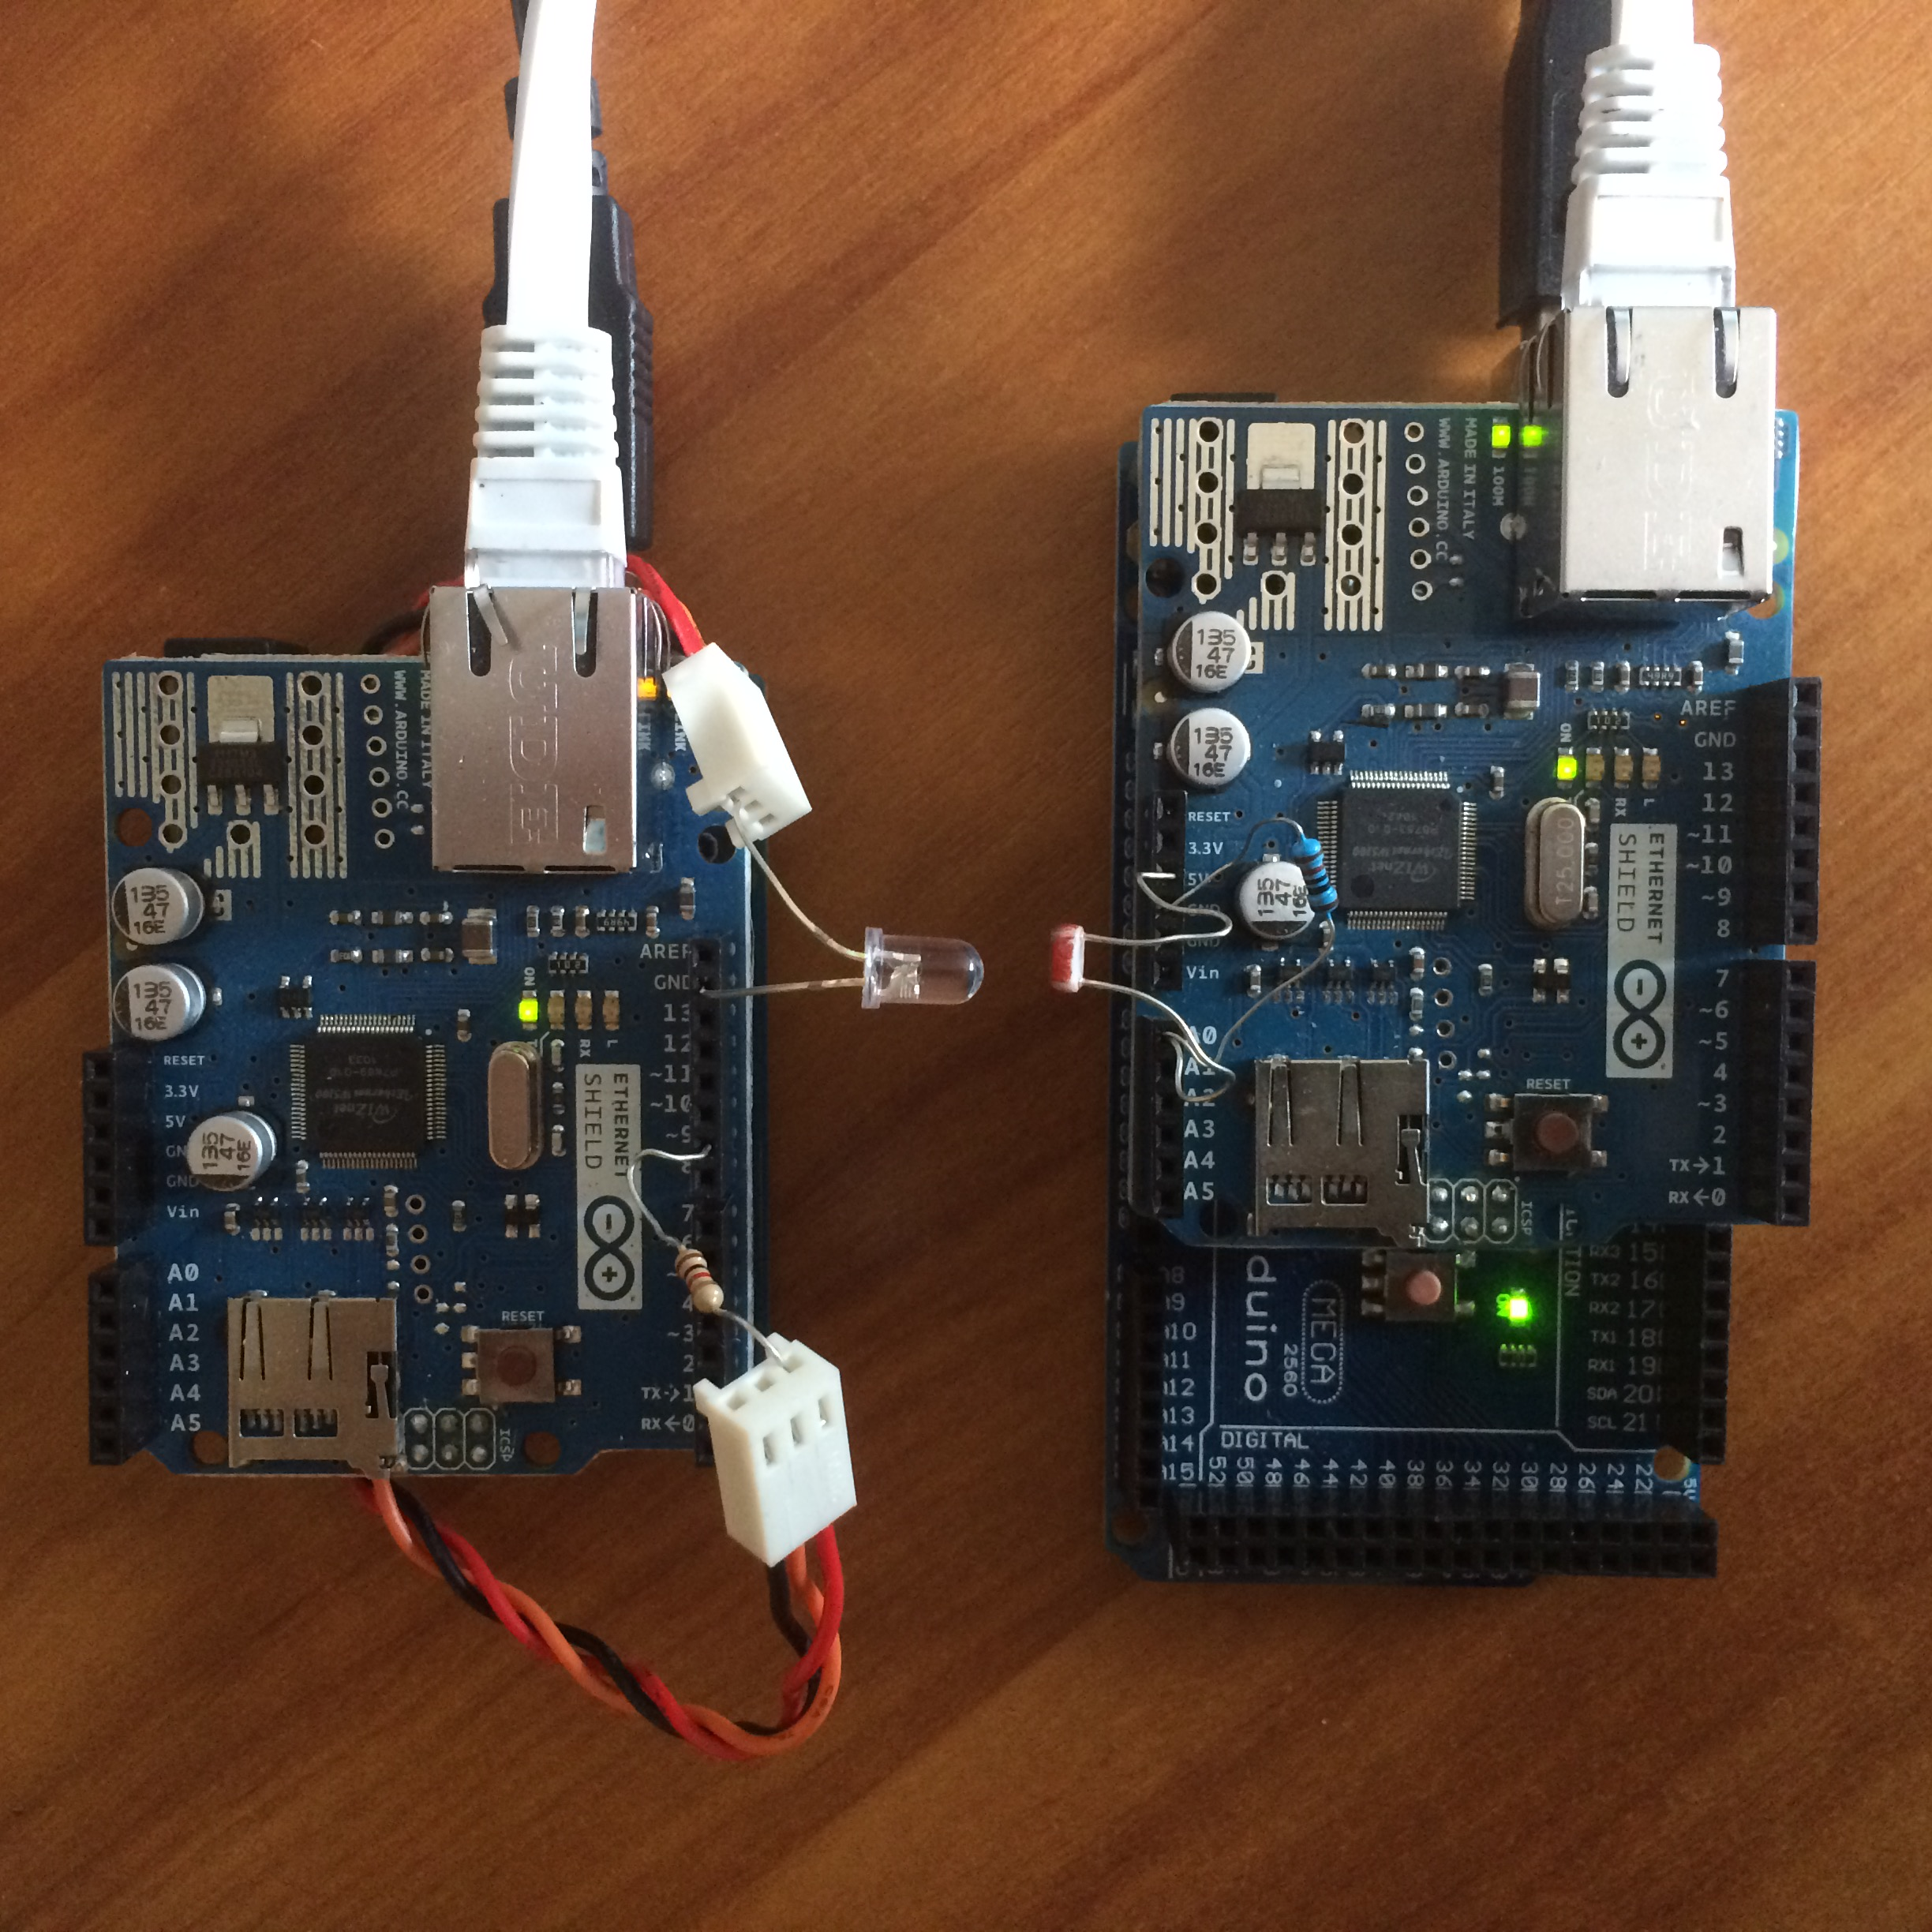
\includegraphics[width=0.5\textwidth]{imp}
  \caption{Prototypes}
  \label{imp}
\end{figure}

\begin{table}[t]
\centering
\caption{\textsc{Performance Evaluation of Device Pairing Protocol}}
\label{evaluation}
{\small
\begin{tabular}{| p{5cm} | p{3cm} |}
 \hline
\textbf{Function} & \textbf{Time(ms)} \\ \hline \hline
Generating Keys & 3898 \\ \hline
commitment Calculation & 15 \\ \hline
commitment Validation & 15 \\ \hline
Transferring OOB message & 3201 \\ \hline
Complete Protocol & 21760 \\ \hline
\end{tabular}
}
\end{table}

\section{Flaws Found in Some Pairing Protocols}

In this section, we are going present flaws that we have found in some pairing protocols. These flaws have not revealed in any publication before. 

We will explain clearly how come we can discover these attack in the next chapter. Briefly speaking, we constructed a formal model to analyse our protocol, and adapted it to do other existing device pairing ones introduced in this chapter. As a result of that, some flaws have been discovered. 

To begin with, we would like to take some assumptions on channels, attacker capabilities, and user actions as below. 
\begin{itemize}
\item Two participants don't play the protocol concurrently.
\item The protocol replays when it accidentally gets an error. 
\item Attacker knows OOB message content before the message is delivered.
\item Attacker can delay user's actions. 
\end{itemize}

Furthermore, protocols are considered in theoretical perspective where OOB channels are classified in our category. In particular, these following protocols are assumed to use long-range public out-of-band channels which only provide channel origin authentication.  

\subsection{Attack on Wong-Stajano Protocol using Bidirectional Channel}

The Wong-Stajano protocol using bidirectional channel was presented at~\ref{WS} in this chapter. The protocol aims to provide a key agreement between two participants. However, we found a counterexample in which the protocol goal does not hold for the initiator. The counterexample is illustrated in the figure~\ref{WSbiattack}, and is precisely detailed in table~\ref{WSbiattacktable}. 

\begin{table}[t]
\centering
\caption{\textsc{Attack Scenario Against Initiator's Guarantee in Wong-Stajano Protocol with Bidirectional Channel}}
\label{WSbiattacktable}
{\small
\begin{tabular}{| l | p{11cm} |}
 \hline
 Step 1.1 & Attacker suspends the $r_b$ sent by $Bob$ on OOB channel\\ \hline
 Step 1.2 & Attacker drops the $K_B$ sent by $Bob$. \\ \hline
 Step 1.3 & Attacker starts a new session with Alice\\ \hline \hline
 Step 2.1 & $Alice$ sends $(A, g^{a}, MAC_{K_{A2}}(A,g^{a},r_{A2}))$ to the Attacker on wireless channel\\ \hline
 Step 2.2 & Attacker sends $(B, g^{x}, MAC_{K_X}(B,g^{x},r_{B}))$ on wireless channel\\ \hline
 Step 2.3 & Attacker drops $R_{A2}$ sent by $Alice$ on OOB channel\\ \hline
 Step 2.4 & Attacker releases $r_b$ at Step 1.1 on OOB channel \\ \hline
 Step 2.5 & Attacker sends $K_X$ to $Alice$ on wireless channel\\ \hline
 Step 2.6 & At the end of the execution, $Alice$ believes she shares a fresh session key with Bob, known actually by the Attacker\\ \hline
\end{tabular}
}
\end{table}

\begin{figure}
  \centering
  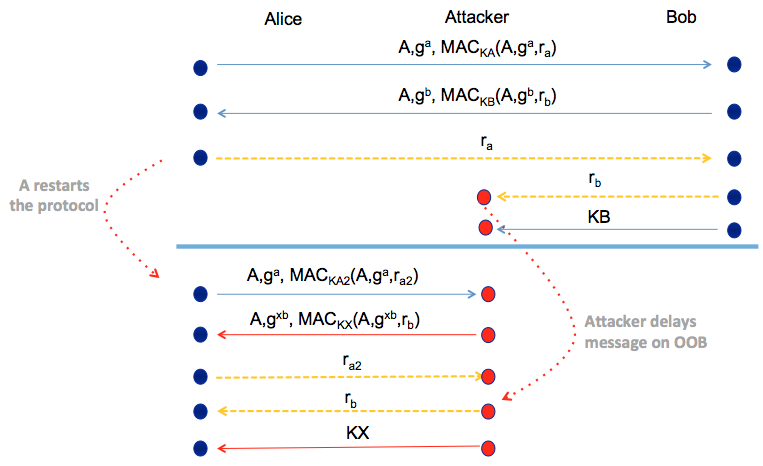
\includegraphics[width=0.9\textwidth]{WSbi}
  \caption{Attack on Wong-Stajano Protocol using Bidirectional Channel with Unidirectional Channel}
  \label{WSbiattack}
\end{figure}

Additionally, we found the protocol is being used in the Pico system of the authors~\cite{Stajano:2014aa}. 
 
\subsection{Attack on Wong-Stajano Protocol using Unidirectional Channel}

The counterexample of Wong-Stajano protocol using unidirectional channel is illustrated in the figure~\ref{WSuniattack}, and is precisely detailed in table~\ref{WSuniattack}. 

\begin{table}[t]
\centering
\caption{\textsc{Attack Scenario Against Initiator's Guarantee in Wong-Stajano Protocol with Unidirectional Channel}}
\label{WSuniattack}
{\small
\begin{tabular}{| l | p{11cm} |}
 \hline
 Step 1.1 & Attacker intercepts $g^{a}$ sent by $Alice$ on wireless channel\\ \hline
 Step 1.2 & Attacker replies with $(B, g^{x}, h_{K_X}(B,g^{x},g^a,r_x))$ to $Alice$ on wireless channel\\ \hline
 Step 1.3 & Attacker suspends $r_b$ sent by $Bob$ on OOB channel, and starts a new session with Alice\\ \hline \hline
 Step 2.1 & $Alice$ sends $g^{a'}$ on wireless channel\\ \hline
 Step 2.2 & Attacker responds $(B, g^{x}, h_{K_X}(B,g^{a'},g^{x'},r_b))$ on wireless channel\\ \hline
 Step 2.3 & Attacker drops $ACK$ sent by $Alice$ on OOB channel\\ \hline
 Step 2.4 & Attacker release $r_b$ sent by $Bob$ on OOB channel at Step 1.3\\ \hline
 Step 2.5 & Attacker sends $K_X$ to $Alice$ on wireless channel\\ \hline
 Step 2.6 & At the end of the execution, $Alice$ believes she shares a fresh session key with $Bob$, known actually by the Attacker\\ \hline
\end{tabular}
}
\end{table}

\begin{figure}
  \centering
  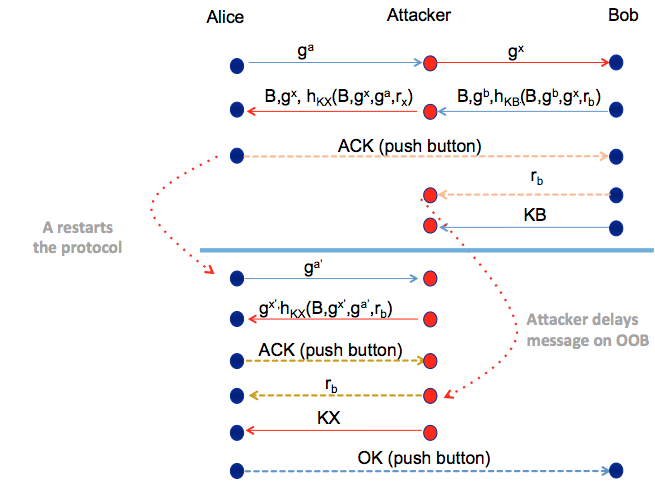
\includegraphics[width=0.8\textwidth]{WSuni}
  \caption{Attack on Wong-Stajano Protocol using Unidirectional Channel}
  \label{WSuniattack}
\end{figure}

\subsection{Attack on SRS-AKA Protocol}

Attack against SRS-AKA is closely identified with one in Wong-Stajano protocol using unidirectional channels. The attack scenario is illustrated in figure~\ref{SRSattack} and detailed at table~\ref{SRSattacktable}.

\begin{table}[t]
\centering
\caption{\textsc{Attack Scenario Against Initiator's Guarantee in SRS-AKA Protocol}}
\label{SRSattacktable}
{\small
\begin{tabular}{| l | p{11cm} |}
 \hline
 Step 1.1 & Attacker intercepts $PK_A$ sent by $Alice$ on wireless channel\\ \hline
 Step 1.2 & Attacker replies with $h(PK_A,PK_X,r_x,SRS_X), PK_X$ to $Alice$ on wireless channel\\ \hline
 Step 1.3 & Attacker suspends $SRS$ sent by $Bob$ on OOB channel, and starts a new session with $Alice$\\ \hline \hline
 Step 2.1 & $Alice$ sends $PK_A$ on wireless channel\\ \hline
 Step 2.2 & Attacker responds $h(PK_A,PK_X,r_x,SRS), PK_X$  on wireless channel\\ \hline
 Step 2.4 & Attacker release $SRS$ sent by $Bob$ on OOB channel at Step 1.3\\ \hline
 Step 2.5 & Attacker sends $r_x$ to $Alice$ on Wireless channel\\ \hline
 Step 2.6 & At the end of the execution, $Alice$ believes she shares a fresh session key with Bob, known actually by the Attacker\\ \hline
\end{tabular}
}
\end{table}

\begin{figure}
  \centering
  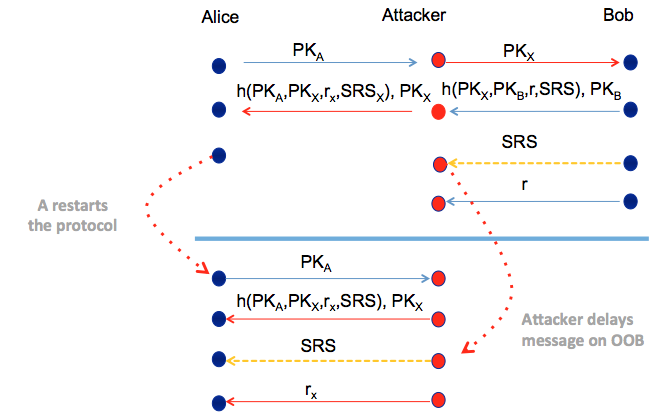
\includegraphics[width=0.8\textwidth]{SRS}
  \caption{Attack Against SRS-AKA Protocol}
  \label{SRSattack}
\end{figure}


\subsection{Attack on Hoepman AKA Protocol}

Since the Hoepman protocol is quite similar to Wong-Stajano protocol with bidirectional channel, the attack found on Wong-Stajano protocol might be used against Hoepman one. But, the difference between two protocols is while two random numbers are exchanged over OOB channel in Wong-Stajano, two short short-hashing values are used in Hoepman version. This apparently lets the attacker a big challenge to break the Hoepman protocol. Nevertheless, due to the less strong hash function, if the attack can find a collision of the short hash function in polynomial time, it is definitely able to launch MITM attack. We take this assumption and present the attack scenario in figure~\ref{Hoepman}, and table~\ref{Hoepmantable}. 
   
\begin{figure}
  \centering
  \includegraphics[width=0.9\textwidth]{Hoepman}
  \caption{Attack Against Hoepman-AKA Protocol}
  \label{Hoepman}
\end{figure}

\begin{table}[t]
\centering
\caption{\textsc{Attack Scenario Against Initiator's Guarantee in Hoepman Protocol}}
\label{Hoepmantable}
{\small
\begin{tabular}{| l | p{11cm} |}
 \hline
 Step 1.1 & Attacker suspends the $S\_h(g^b)$ sent by $Bob$ on OOB channel\\ \hline
 Step 1.2 & Attacker finds $g^x$ so that $S\_h(g^x) = S\_h(g^b)$. It does not necessary to find $h(g^x) = h(g^b)$  \\ \hline
 Step 1.3 & Attacker starts a new session with Alice\\ \hline \hline
 Step 2.1 & $Alice$ sends $h(g^{a2})$ to the Attacker on wireless channel\\ \hline
 Step 2.2 & Attacker sends $h(g^{x})$ to $Alice$ on wireless channel\\ \hline
 Step 2.3 & Attacker drops $S\_h(g_{a2})$ sent by $Alice$ on OOB channel\\ \hline
 Step 2.4 & Attacker releases $S\_h(g^b)$ at Step 1.1 on OOB channel \\ \hline
 Step 2.5 & $Alice$ sends $g^{a2}$ to Attacker on wireless channel \\ \hline
 Step 2.6 & Attacker sends $g^{x}$ to $Alice$ on wireless channel\\ \hline
 Step 2.7 & At the end of the execution, $Alice$ believes she shares a fresh session key with Bob, known actually by the Attacker\\ \hline
\end{tabular}
}
\end{table}

\section{Conclusion}

In this chapter, we have conducted a deep survey on out-of-band channel types and secure device pairing protocols. Moreover, we have provided a novel solution to the fundamental issues of key agreement over a radio links. To our knowledge, our proposal requiring only 2 wireless radio messages and one out-of-band message is more economic than existing protocols in term of communication cost. Yet it still provides a security level equivalent to one of existing protocols. We also gave a sketch of proof in a computational model. Additionally, an implement of our protocol has been conducted and tested in an embedded system to show that it is practical via our benchmark. In mean while, we found some flaws of Wong-Stajano protocols, Hoepman protocol, and SRS-AKA protocol, this has not introduced before. 




